\documentclass[lettersize,journal]{IEEEtran}
\usepackage[commandnameprefix=always]{changes}
\usepackage{amsmath,amsfonts}
\usepackage{algorithmic}
\usepackage{algorithm}
\usepackage{array}
\usepackage{subfigure} 
\usepackage[caption=false,font=normalsize,labelfont=sf,textfont=sf]{subfig}
\usepackage{textcomp}
\usepackage{stfloats}
\usepackage{url}
\usepackage{verbatim} 
\usepackage{graphicx}
\usepackage{cite}
\usepackage{booktabs}
\usepackage{multirow}
\usepackage{makecell}
\usepackage{color}
\usepackage{tabularray}
\usepackage{tabularx}
\usepackage{url}


\hyphenation{op-tical net-works semi-conduc-tor IEEE-Xplore}


\begin{document}


\title{A Comprehensive Survey on Orbital Edge Computing: Systems, Applications, and Algorithms}

\author{Changhao Wu,~\IEEEmembership{Student Member,~IEEE},
Yuanchun Li,~\IEEEmembership{Member,~IEEE},

Mengwei Xu,~\IEEEmembership{Member,~IEEE},
Chongbin Guo,~\IEEEmembership{Member,~IEEE},

Zengshan Yin, Weiwei Gao, and Chuanxiu Chi


\thanks{
  This work was supported in part by Shanghai Rising-Star Program under Grant 19QA140800, Youth Innovation Promotion Association for CAS under Grant 2019292, and in part by The Hong Kong, Macau, and Taiwan Science and Technology Cooperation Project in the ``Science and Technology Innovation Plan Of Shanghai Science and Technology Commission" under Grant 23510760200. (Corresponding author: Chongbin Guo)
  


  Changhao Wu, Chongbin Guo and Zengshan Yin both are with Innovation Academy for Microsatellites of Chinese Academy of Science, Shanghai 201304, China, and University of Chinese Academy of Sciences, Beijing 101408, China (e-mail: jacob626@126.com). 

  Yuanchun Li are with Research Assistant Professor at the Institute for AI Industry Research, Tsinghua University, Beijing 100084, China.
  
  Mengwei Xu, Weiwei Gao and Chuanxiu Xi are with State Key Laboratory of Networking and Switching Technology Computer Science Department, Beijing University of Posts and Telecommunications, Beijing 100876, China. 

}% <-this % stops a space
% \thanks{Manuscript received April 19, 2021; revised August 16, 2021.}
}

% The paper headers
\markboth{}%
{Shell \MakeLowercase{\textit{et al.}}: A Sample Article Using IEEEtran.cls for IEEE Journals}

\IEEEpubid{}
% Remember, if you use this you must call \IEEEpubidadjcol in the second
% column for its text to clear the IEEEpubid mark.

\maketitle


\begin{abstract}

The number of satellites, especially those operating in low-earth orbit (LEO), is exploding in recent years. Additionally, the use of COTS hardware into those satellites enables a new paradigm of computing: orbital edge computing (OEC). OEC entails more technically advanced steps compared to single-satellite computing. This feature allows for vast design spaces with multiple parameters, rendering several novel approaches feasible. The mobility of LEO satellites in the network and limited resources of communication, computation, and storage make it challenging to design an appropriate scheduling algorithm for specific tasks in comparison to traditional ground-based edge computing. This article comprehensively surveys the significant areas of focus in orbital edge computing, which include protocol optimization, mobility management, and resource allocation. This article provides the first comprehensive survey of OEC. Previous survey papers have only concentrated on ground-based edge computing or the integration of space and ground technologies. This article presents a review of recent research from 2000 to 2023 on orbital edge computing that covers network design, computation offloading, resource allocation, performance analysis, and optimization. Moreover, having discussed several related works, both technological challenges and future directions are highlighted in the field.
\end{abstract}

\begin{IEEEkeywords}
Orbital edge computing, Computation offloading, Resource allocation, Mobility management.
\end{IEEEkeywords}

\section{Introduction}
\label{sec1}
\IEEEPARstart{C}{loud} computing has become a new paradigm of computing in the terrestrial network, which has recently emerged as a commercial reality \cite{RN143}. In recent years, moving computation load to network edges has shown to reduce the latency and energy cost of the network. Moreover, mobile edge computing (MEC) is well adapted to computation-intensive and latency-critical tasks on mobile devices \cite{SN1}. Recent research has agreed that MEC is a critical technology for realizing various visions for next-generation Internet, such as Internet of Things (IoT) \cite{RN141}, Internet of Vehicles (IoV) \cite{RN257,RN72} and 6th generation mobile network (6G) \cite{RN142}. 

LEO satellite network is a promising technology due to its ubiquity and invulnerability \cite{RN77}. To address this issue, large-scale low earth orbit (LEO) satellite network has been extensively investigated \cite{RN88}. Currently, several LEO satellite projects aimed at providing global communication have been launched, such as OneWeb \cite{RN144}, SpaceX Starlink \cite{RN146} and O3b \cite{RN147}. Large-scale constellations hold great potential to enable computation-intensive services on the ground and in space \cite{RN77}. Moreover, the LEO satellite network can also support computation services from users in remote areas and from the ocean \cite{RN255}. Therefore, it is highly demanding to deploy MEC in satellite network to meet the needs of emerging applications, such as augmented reality (AR)/virtual reality (VR), high definition (HD) video transmission, and autonomous driving \cite{RN55}. Furthermore, orbital tasks such as remote sensing and space domain awareness (SDA) \cite{RN148} generate a massive amount of data every moment, which demands powerful computation power to support the massive data generation and  mitigate the bottlenecked communication between the ground and space \cite{RN13}.


\IEEEpubidadjcol

\begin{figure}
  \centering
  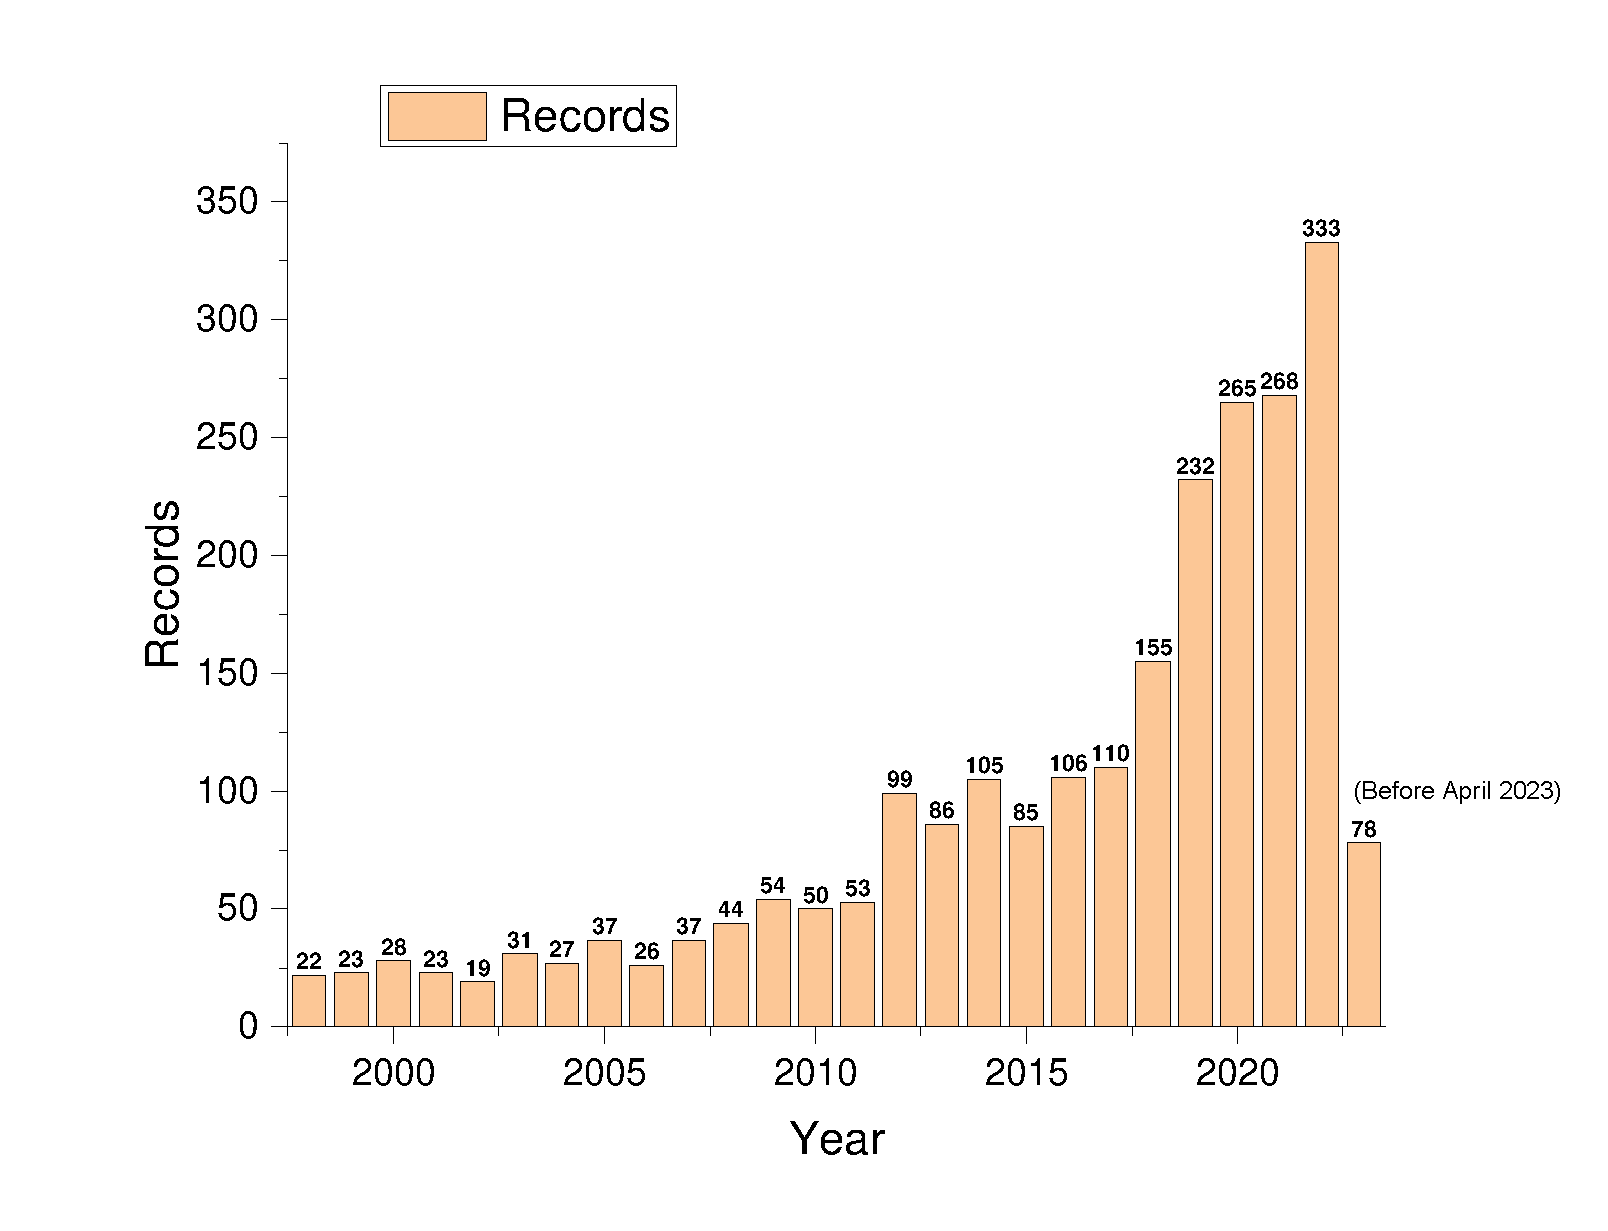
\includegraphics[width = 0.48\textwidth]{fig2.pdf}
  \caption{The statistical analysis of the research trend in OEC. ``Records" indicate the number of articles related to OEC retrieved by ``Web of Science" in the given year.}
  \label{Fig1}
\end{figure}

In earlier years, software-defined network (SDN) technology abstracted network resources to virtualized systems, making network resources easier to manage, and subsequently promoting the development of cloud computing. As an important component of communication network, the concept of integrating virtual information resources from satellites and the Internet was proposed by Kanev et al. \cite{RN180}, which initiated wide concerns about satellite cloud computing. However, due to harsh communication conditions and the high cost of launch, the application scenarios of satellite cloud computing are limited. 

With the development of nano-satellite technology and the LEO satellite industry, the launching cost of satellites has been greatly reduced, and the computing capability of satellites has been significantly improved. Benefited by the large number of satellites, edge computing offers better potential over cloud computing as it can alleviate the pressure on satellite communication. The first concept and architecture of OEC were proposed by Bradley et al. from Carnegie Mellon University in 2019 \cite{RN57, RN180}. This work validates that OEC improves the efficiency of remote sensing image processing by avoiding redundant data transmission between satellites and the ground. Currently, OEC has been considered a promising technology in various applications. For example, remote sensing image information captured by LEO satellites can be processed directly by OEC, and reducing the amount of data that needs to be transmitted back to the ground.


In recent years, researchers from industry and academia have investigated a wide range of issues related to OEC, including satellite networking \cite{RN88}, research platform \cite{RN13}, testbed \cite{RN102}, architecture \cite{RN55, RN56}, resource management \cite{RN58} and computation offloading strategy \cite{RN16, RN43}. Fig. \ref{Fig1} provides the statistics on the number of research articles on the keyword ``satellite edge computing" over the past 25 years. The explosion of research in the last decade has highlighted the great potential of OEC. 

\begin{figure*}
  \centering
  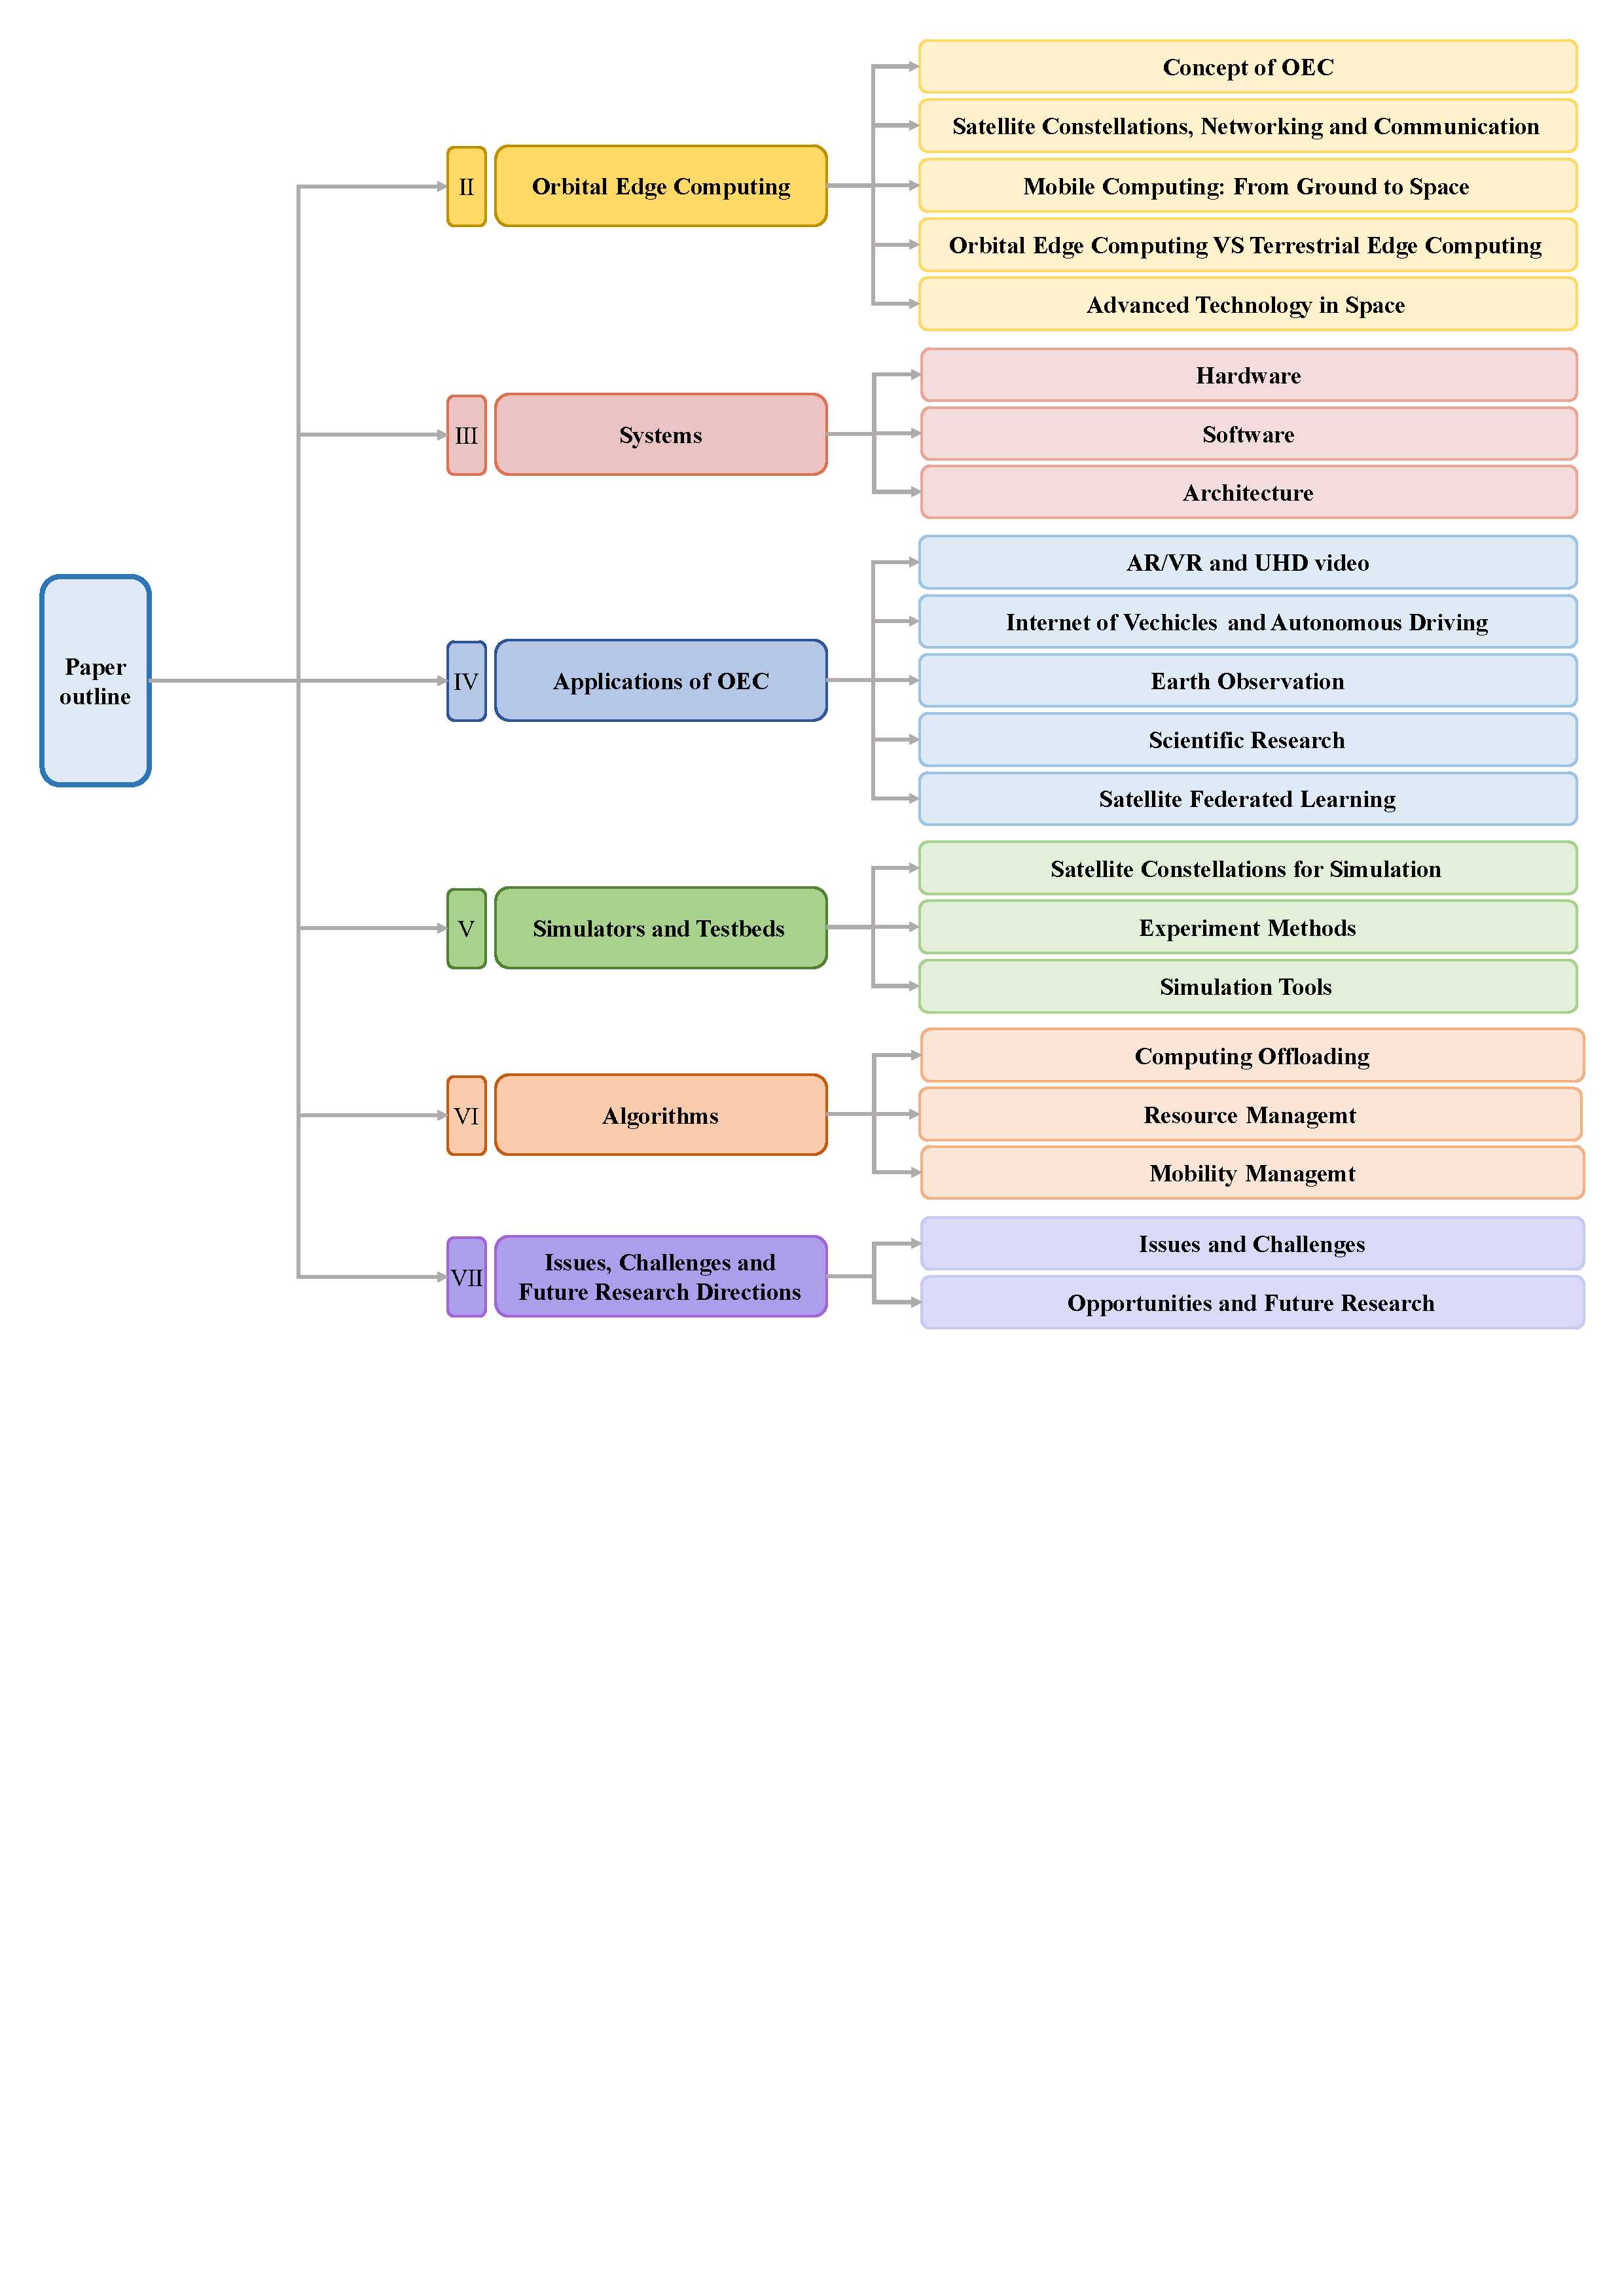
\includegraphics[width = 0.8\textwidth]{fig1.pdf}
  \caption[c]{The outline of this paper.}
  \label{Fig4}
\end{figure*}   

Several survey articles have been published to provide overviews of the MEC. However, OEC is still a concept that only several experimental satellites have been launched for verification. There is still a lack of a systematic survey article providing a comprehensive discussion on OEC. In this paper, we presents a literature survey on the OEC field from 2000 to 2023, and provides an overview of key research progress that includes satellite networking, resource management, and computation offloading in this new field. In Section \ref{sec2}, we firstly introduce the OEC concept, background, and advanced space technology, and comparison between it and MEC in the terrestrial network. Next, various applications of OEC are summarized in Section \ref{sec3}. Subsequently, we conclude the testbed and experiment methods of OEC in \ref{sec4}. After that, Section \ref{sec5} summarizes the algorithms in OEC, focusing on resource management, movability management, and computation offloading. Finally, Section \ref{sec6} concludes key research issues and future directions.

\section{Orbital Edge Computing}
\label{sec2}
In this section, we first introduce the concept and background of OEC. Second, we introduce the satellite constellations and networking, which are the basis of OEC architecture. Third, we introduce the evolution of OEC from ground-based mobile computing. Next, we compare the orbital edge computing to terrestrial mobile edge computing. Finally, advanced technologies in space such as laser communication, smart satellites and space-air-ground integrated network are introduced.

\subsection{Concept of OEC}
OEC is a network architecture where computing resources are pushed to satellites. Traditionally, satellites act as data sources in the network and transmit the raw data to the ground based on a bent-pipe architecture. In OEC network architecture, satellites are equiped with computing capabilities, which can complete various computing tasks as edge nodes in the network. Due to the computation resources are located closer to the data source, OEC greatly improves the communication performance of the network by processing sensor data in orbit. OEC provide more diversified services, such as on-orbit data preprocessing, real-time remote sensing image analysis and disaster monitoring. 

\subsection{Satellite Constellations, Networking and Communication}


\begin{table*}[htbp!]
  \centering
  \caption{COMPARISON OF SATELLITES IN DIFFERENT ORBIT  \cite{TN927} } 
  \label{tab-1}
  \begin{tabular}{ccccc} \hline
              & Low Earth Orbit (LEO) & Highly Elliptical Orbit (HEO)  & Middle Earth Orbit (MEO)  & Geostationary Orbit (GEO)\\ \hline % 卫星类型
  Inclination & \makecell[c]{80 $\sim$ 95$^\circ$ (near-polar orbit) \\45 $\sim$ 60$^\circ$ (inclined orbit)}   &  63.4$^\circ$  & 45 $\sim$ 60$^\circ$ & 0$^\circ$ \\ \hline      % 倾角

  Altitude & \makecell[c]{300 $\sim$ 1500 km}   &  \makecell[c]{600 $\sim$ 40000 km}  & \makecell[c]{8000 $\sim$ 20000km} & 35786 km \\ \hline      % 高度

  Period & 1.4 $\sim$ 2.5 hours &  12 hours & 6 $\sim$ 12 hour & 24 hours \\ \hline      % 周期
  \makecell[c]{Number of satellites \\ in a constellation} & 24 $\sim$ thousands   &  4 $\sim$ 8 & 8 $\sim$ 16 & 3 $\sim$ 4\\ \hline      % 每星座周期数

  Coverage & Global    &  High latitude areas  & Global & Global (except polar regions) \\ \hline      % 覆盖

  Latency & 5 $\sim$ 35 ms &  150 $\sim$ 250 ms & 50 $\sim$ 100 ms & 270 ms \\ \hline      % 时延

  Pass durations  & About 10 minutes   &  4 $\sim$ 8 hours & 1 $\sim$ 2 hours & All the time \\ \hline      % 过顶时间

  % \makecell[c]{Data rates \\ } & 3.75Gbps    & Unknown  &  1.2Gbps & 87kbps \\ \hline      % 数据速率

  Typical constellation & \makecell[c]{Iridium, Starlink, \\Kuiper, O3B}    & \makecell[c]{Molniya, Loopus, \\Archimedes}  & \makecell[c]{Odyssey}& \makecell[c]{Inmarsat, MSAT\\ Mobilesat} \\ \hline      % 典型系统
  \end{tabular}
\end{table*}
 

\subsubsection*{Satellite Constellation}

A satellite constellation is a group of artificial satellites working together as a system. Satellites in a constellation have similar parameter such as orbit altitude and orbit inclination. Satellite constellations can provide superior coverage and lowered launch costs. Additionally, they offer unique communication and coverage performance that varies according to the orbital altitude. These distinctions are made clear through Table \ref{tab-1}. GEO satellite-backed Internet access has been available for decades as they have the advantage of the wide coverage, which can achieve global communication with only three satellites (the small regions around the North and South Poles are normally excluded). However, The high altitude and the requirement to orbit above the equator result in high access latency for consumers, which renders satellite Internet infeasible  for many use cases \cite{RN168, RN169}.   

\begin{figure}
  \centering
  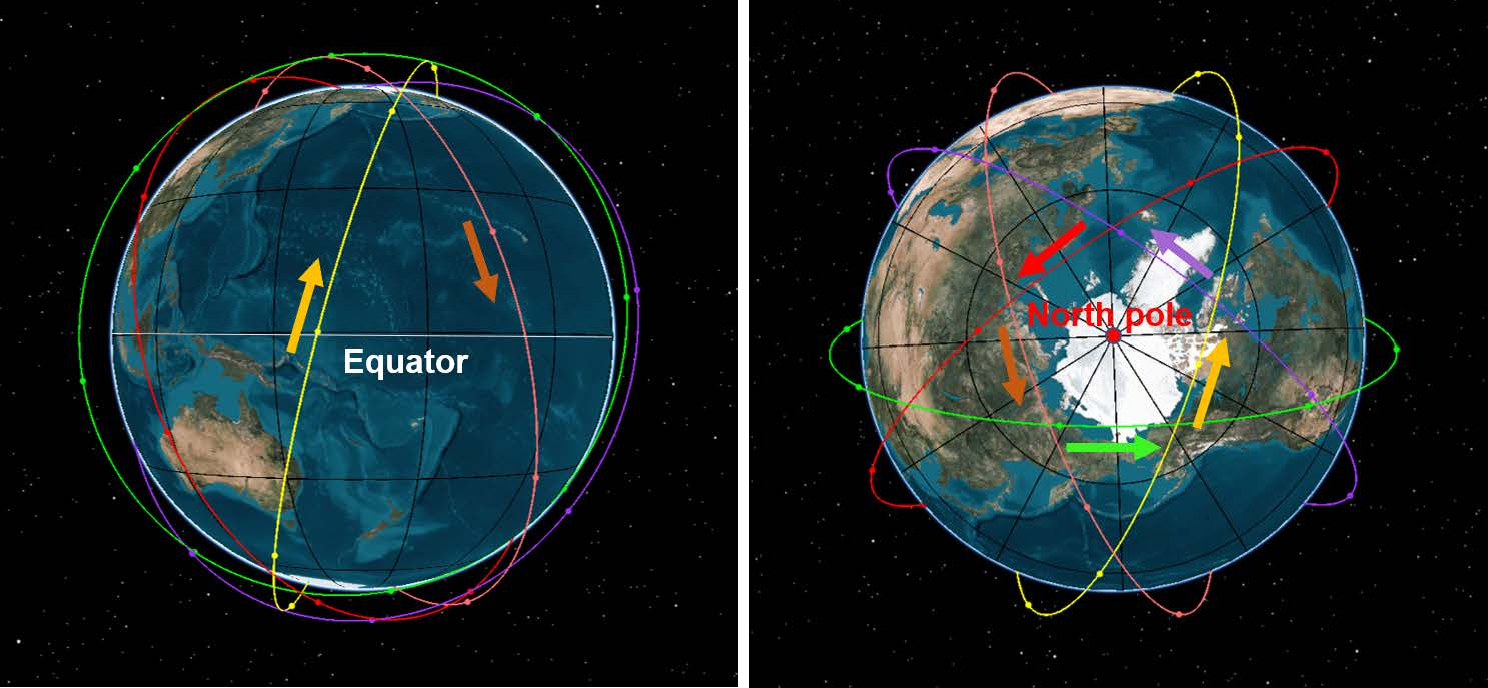
\includegraphics[width = 0.48\textwidth]{fig7.pdf}
  \caption{Illustration of a $75^\circ:40/5/1$ Walker $\delta$ constellation, at an altitude of 800 km.}
  \label{fig:7}
\end{figure}

The development of mobile communication motivates improvement in satellite communication with better performance. LEO satellites attract research attentions due to its better latency and lower launch cost. In 1997, the Iridium constellation was launched to provide voice and message communication service \cite{RN194}. It consists of 66 active satellites in orbit at a height of approximately 781 kilometres and inclination of $86.4^\circ$. Iridium constellation has a remarkable characteristic in which satellites can keep relative stability to each other even in different orbit planes. In providing telephone service, the user has a shorter range to non-GEO satellite network, therefore, less radiated power is required, and the propagation delay is reduced \cite{RN197}. However, one major drawback of the Iridium constellation is its uneven coverage density, high latitude area can enjoy more dense coverage while it becomes more and more sparse with the latitude lowers. On the other hand, the Walker satellite constellation \cite{RN195} can realize global uniform coverage, but satellites from different orbit planes cannot maintain a static formation. The Walker constellation is defined by $i:t/p/f$, where $i$ is the inclination, $t$ the total number of satellites and $p$ the number of orbit planes. The phase parameter $f$ is the relative spacing between satellites in adjacent planes. In particular, the Walker constellation is divided into two types: star and delta. The former comprises near-polar orbits at an inclination angle of about 90 degrees. Conversely, the latter includes orbits at an inclination angle generally less than 60 degrees, with the ascending node of the plane distributed over the full range of 360 degrees, and the satellites spaced evenly on the orbit. Emerging massive constellations such as Starlink and Kuiper follow the design of the Walker delta constellation. An example of $75^\circ:40/5/1$ Walker $\delta$ constellation is shown as Fig. \ref{fig:7}. 


\subsubsection*{Satellite Communication} 
Frequency is a crucial factor for satellite communication, microwave (300MHz-300GHz) is suited to satellites because of its wide bandwidth and high frequencies as well as the ability to use small antennas. Table \ref{tab4} shows the frequency bands used by satellites. Most communication satellites work in the $C$ frequency band, and with an up link frequency of 5.925 to 6.425GHz and a downlink frequency of 3.7 to 4.2GHz. At present, the $X$, $Ku$ and $Ka$ frequency band has been developed for civil service and broadcasting. However, scarce radio frequency bands cannot keep pace of the rapid increase of satellite applications. Higher frequency bands, such as the $V$ frequency, even up to the optical frequency range (190THz to 560THz), are being explored. For example, Starlink \cite{SpaceXNews} and Micius Satellite \cite{lu2022micius} has equipped with laser communication payload. 

\begin{table}[htbp!]
  \centering
  \caption{Frequency bands used by satellites and their code}
  \label{tab4}
  \begin{tabular}{ccc} \hline
  \textbf{Code} & \textbf{Frequency band} & \textbf{Used by Satellites (down-link/up-link)} \\ \hline
  UHF & 300MHz to 3GHz & 400/200MHz \\
  $L$ & 1GHz to 2GHz & 1.6/1.5GHz \\
  $C$ & 4GHz to 8GHz & 6/4GHz \\
  $X$ & 4GHz to 8GHz & 8/7GHz \\
  $Ku$ & 12GHz to 18GHz & 14/12GHz, 14/11GHz \\
  $Ka$ & 27GHz to 40GHz & 30/20GHz \\ 
  $V$ & 40GHz to 75GHz & 50/40GHz \\ \hline
  \end{tabular}
\end{table}

In recent years, thousands of small satellites have been deployed in mega constellations at altitudes below 600 km, i.e., in the LEO. Thus, 
LEO constellations can also achieve global and continuous coverage thanks to its large number \cite{RN170,RN171}. However, low altitude orbits incur short-time connections between satellites and ground stations (tens of minutes). Inter-satellite communication performs better, especially long-distance, because light propagates faster in a vacuum than in fiber \cite{RN172}. Inter-satellite links (ISLs) include intra-orbit and inter-orbit links \cite{RN218}. Intra-orbit links connect satellites in the same orbit plane and form a stable ring network. Satellites in one ring network keep a relatively stationary position with each other. Instead, inter-orbit links connect satellites across orbit planes. In the Walker constellation, inter-orbit links are time-variant. The link between satellites can only keep for a short time.  

\subsubsection*{Satellite Network Topology Modeling}
A satellite network is a dynamic network composed of nodes and links. In this network, nodes are satellites, and links are the communication links between nodes. Due to the time-variant positions of satellite, the network topology is changing continuously. In the Walker constellation, links between satellites can only survive about ten or twenty minutes which depends on the satellite's orbit. In this subsection, we summarize the algorithm for modeling the topology of a satellite network by refering to \cite{RN196}.

Assuming the links in the network will be broken only if the two satellites are out of sight. The node can be modeled as $S=\{N,P\}$, where $N$ is the identifier of the satellite and $P$ is the position in space. The describe of position could be orbit or coordinates. The model of link $L=\{N_{S1},N_{S2},t_s,t_e\}$ describes the identity of the two satellites $N_{S1},N_{S2}$ and the time $t_s$, $t_e$ when the link is built and broken. Naturally, the difference $t_l=t_e-t_s$ represents the survival time of the link.

In fact, the topology change of the satellite communication network occurs at some specific moment. Therefore, the time of the simulation model could be discrete. In \cite{RN196}, the topology is fixed during a period which is called timeslice $T_i=[T_{si},T_{ei}](i=1,2,3\ldots)$, where $T_i$ is the $i$-th timeslice in the simulation time and $T_{si}$ is the time at which it starts and $T_{ei}$ is the time it ends. Naturally, $T_{s(i+1)} = T_{ei}$. Based on this, the time-variant topology can be modeled like $G_d=\{T,\{S_1,S_2,\ldots,S_M\},\{T_1,T_2,T_3,\ldots\},\{G_{s1},G_{s2},G_{s3},\ldots\}\}$, where $T$ is duration of simulation time. $\{S_1,S_2,\ldots,S_M\}$ is the set of satellite nodes and $M$ is the total number of them. In the $i$-th timeslice, the model $G_{si}(i=1,2,3\ldots)$ describes the satellites(nodes) and links as $G_{si}=\{T_i,\{ S_{i1},S_{i2},\ldots,S_{im} \},\{L_{i1},L_{i2},\ldots,L_{in}\} \}$. It indicates that in the $i$-th timeslice, there are $m$ satellites bulit $n$ links. The nodes are $\{ S_{i1},S_{i2},\ldots,S_{im} \}$ and links are $\{L_{i1},L_{i2},\ldots,L_{in}\}$. Based on this model, the network topology is a dynamic graph, and some algorithms of OEC, such as computation offloading, mobility management, and resource allocation, can be simulated. Furthermore, the weight of links in this model can be defined according to particular needs.

\subsection{Mobile Computing for IoT: From Ground to Space}
Over the last decade, the proliferation of mobile devices has facilitated remarkable progress in IoT and 5G/6G communication. The notion of IoT, which refers to the ability of computers to sense information without human intervention, has been extensively applied to diverse domains, including healthcare, environmental monitoring, home automation, and transportation \cite{RN152,RN154}. With the burgeoning number of smart terminals, a massive volume of data is generated incessantly. Fortunately, sophisticated communication technologies, comprising optical-fiber and wireless communication, enable cloud-based computing and storage services at a remote data center.

Nowadays, some extreme applications such as AR/VR, ultra-HD (UHD) video streaming, and autonomous driving require extremely low latency or enormous computation ability, even both, which could be a heavy load for network and cloud services. Cloud computing will not be efficient enough to support these applications \cite{RN150}. Hence, In 2014, mobile edge computing was first proposed by the \emph{European Telecommunications Standard Institute} (ETSI) to mitigate the pressure of cloud computing and supply lower latency of network \cite{RN155}. 

However, due to the limited coverage, the terrestrial network cannot provide seamless access, especially in remote areas (such as deserts, forests, oceans, etc.). With the cost of satellite manufacturing and launching reduced, the space-air-ground integrated network is expected to play a pivotal role in IoT \cite{RN88}. Subsequently, to address the limitations of a bent-pipe architecture, OEC was first proposed in \cite{RN187}. By organizing a set of nanosatellites that orbit on the same path (i.e., flying in formation) into the pipelines that parallelize both data collection and data processing, OEC can reduce ground infrastructure and system edge processing latency compared to a bent-pipe architecture. Similarly, the paper \cite{RN57} describes power and software optimizations for the OEC based on this formation flying architecture. This work has verified the feasibility of distributed computing in space. After the concept of space distributed computing was proposed, inter-satellite communication and on-board processing capability have become bottlenecks. Fortunately, edge computing is implemented on a virtualized platform, allowing high-bandwidth and low-latency applications while decreasing privacy and security risks as well \cite{RN157,RN158}. Moreover, OEC has been verified to support more advanced computing in space \cite{RN187}.


\subsection{Orbital Edge Computing Versus Terrestrial Edge Computing}
As shown in Table \ref{tab1}, there exist significant disparities between OEC and MEC systems in terms of hardware, communication, etc. Compared with MEC, OEC has the advantage of achieving more extensive and even coverage. More advantages are briefly described through some examples and applications in the following.

\begin{table*}[htbp!]
  \centering
  \caption{COMPARISON OF OEC AND MEC SYSTEM}
  \label{tab1}
  \begin{tabular}{ccc} \hline
                  & OEC & MEC \\ \hline
  Server location & LEO, GEO, Ground station  &  Base stations \cite{RN167} \\ \hline    
  Coverage        & 100\%                     &  20\% \cite{RN4}  \\ \hline  % 地面网络的覆盖率
  Mobility        & Predictable               & Random                       \\ \hline 
  Hardware Maintenance   & Hard              &  Easy                           \\ \hline   
  Server hardware & CPU, GPU, FPGA, VPU \cite{RN56}  & \makecell[c]{SoC (smartphone) \\ CPU,GPU (tablet computers) \cite{RN155} } \\ \hline 
  Communication   & \makecell[c]{Wireless communication, \\Laser communicationt}  & \makecell[c]{Wireless communication, \\Optical-fiber communication} \\ \hline % 激光通信
  Application   & \makecell[c]{Autonomous border monitoring \cite{RN55},\\ Space situational awareness\cite{lei2021maddpg}}    & \makecell[c]{AR/VR, Autonomous driving\cite{RN174}, \\ Interactive media and video streaming \cite{RN175}\\}   \\ \hline
  \end{tabular}
\end{table*}

\emph{Coverage:} 
Terrestrial network consists of both fiber and wireless communication, including WiFi, LTE, and 5G, and they can efficiently provide communication services for users in densely populated areas. However, providing internet access to remote regions using terrestrial network can incur substantial costs. In addition, cloud servers and data centers are usually located near metropolitan areas, making it challenging to provide internet access to remote areas \cite{RN102}. Satellites, on the other hand, offer complete coverage with as few as three GEO or 66 LEO satellites (iridium satellite constellation \cite{RN173}) . The higher orbit altitude, the better a single satellite's coverage, and the fewer satellites are needed in a constellation. Satellite network can also offer redundancy for ground-based network, ensuring smooth communication flows even if terrestrial network fails due to power outages. Furthermore, satellites can support remote applications such as smart traffic management and monitoring, making them a suitable option for areas where terrestrial network may not be feasible.


\emph{Latency:} 
The latency for MEC and OEC services is composed of three components: propagation distance, computational capacity, and communication bandwidth. Lower orbit altitude of a satellite results in lower latency due to shorter propagation distance from space to the ground. For instance, Starlink satellite constellation is established in 600 km orbit to achieve latency of under 4ms \cite{RN146}. Additionally, these new satellites can take advantage of inter-satellite laser links for communication, enabling the use of light propagation with a speed of 100 Gb/s or higher, which is about 50\% faster than fiber cables \cite{RN181}. For example, the round-trip time (RTT) for internet communication between New York and London is about 76ms. On the other hand, the minimum RTT achievable via optical fiber that follows a great circle path is 55ms. However, the use of ISLs can further reduce the RTT to only 50ms \cite{RN182}.

\emph{Computing:} 
Due to design constraints, satellite payloads have limited computing power, which is similar to IoT devices in MEC. Therefore, applications are expected to cooperate. It is unclear whether there are any significant differences between OEC and MEC in the learning model. For example, classic deep learning models like Mask R-CNN \cite{he2017mask} have been applied to cloud detection in remote sensing images \cite{RN184}. However, OEC's mobile terminals are smartphones or tablet computers, which are different from those of MEC. Typically, LEO satellites function as mobile terminals, and ground stations (GS) serve as servers in OEC \cite{RN61}. Computing hardware in smartphones consists of System on Chip (SoC), such as the A15 chip in iPhone14, which has six cores based on a 5nm technology node and provides 8.6W of power and 15.8 Tera Operations Per Second (TOPS) \cite{iphone}. Unlike MEC, satellite hardware demands more reliability due to the challenging conditions of space. The first smart satellite funded by the European Space Agency (ESA), called $\Phi$-Sat, carried the Movidius Myriad 2 Video Processing Unit (VPU) \cite{RN185} based on 28nm technology. This VPU, with only 0.98W of power and 2 TOPS, was applied to hyperspectral images for cloud detection based on CNN \cite{RN186}.

\subsection{Advanced Technology in Space}
In the following subsection, we introduce recent advances in technology that could be beneficial to our organization, including laser communication, smart satellites, and space-air-ground integrated network.

% laser ISLs
\subsubsection*{Laser communication} 

The advancements in free space optical (FSO) communication have paved the way for a next-generation technology known as laser communication, which promises to improve communication rates and ranging accuracy in satellite network. Laser ISLs offer significant advantages over traditional microwave communication, including large bandwidth, high data rate, ease and speed of deployability, and low power. The first laser ISLs were demonstrated in 2008 between Terra SAR-X and NFire, two LEO satellites located 5500 km apart and moving at a speed of 25,000 km/h, achieving a capacity of 5.5 Gbps \cite{RN201}. Studies have shown that laser communication technologies are superior to radio frequency (RF) technologies in terms of data rate, secure communication, and weight reduction \cite{RN204,RN205,RN202,RN203}. Table \ref{tab:3} provides a summary of the comparative features between laser and RF communication. One of the most promising applications of laser communication is SpaceX's Starlink project, which plans to use inter-satellite laser communication technology to provide internet services up to 1 Gbps with the deployment of 12,000 satellites \cite{SpaceXNews}.


\begin{table}[htbp!]
  \centering
  \caption{Laser Versus RF for ISLs \cite{RN201}}
  \label{tab:3}
  \begin{tabular}{|c|c|c|}
    \hline
    \textbf{Characteristic} & \textbf{Laser ISLs} & \textbf{RF links} \\ \hline
    Spectrum & \makecell[c]{near infrared and \\ visible light band} & \makecell[c]{Ka, Ku and \\ mm-wave band}\\ \hline
    Bandwidth & in THz & in GHz \\ \hline
    Wavelength & in nm & \makecell[c]{thousands of times larger \\ than the optical wavelength}\\ \hline
    Beam spread & much narrower & typically 1000 times more\\ \hline
    Power consumption & \makecell[c]{more received \\ power for a given \\ transmitted power}& \makecell[c]{less received \\ power for a given \\ transmitted power}\\ \hline
    Security & \makecell[c]{very difficult to \\intercept due to \\ high directivity}& \makecell[c]{easy to intercept}\\ \hline
    Hardware & \makecell{less volume \\ and less weight} & \makecell{more volume \\ and more weight}\\ \hline 
  \end{tabular}
\end{table}

\subsubsection*{Smart satellite}
% 软件定义卫星
A satellite is typically developed for a single or a small number of specific missions, which determine its capabilities, functions, and operations. The integration of hardware and software on a satellite is tightly coupled, making the whole system inflexible and non-universal. However, certain architectural components, such as communication systems and antennas, can be shared between different missions. The software-defined satellite (SDS) has been proposed as a potential solution to the aforementioned challenges, improving satellite network efficiency by using software-defined radio as its universal hardware platform and defining its functions via software \cite{RN199}. China's Chinese Academy of Sciences (CAS) has developed and launched the experimental Tianzhi series of software-defined satellites. The Tianzhi No. 2 D-star is capable of supporting super-resolution image reconstruction on the satellite due to its 40 TOPS computational power and only 19 kg weight. The successful application of SDS has facilitated the development of smart satellites. However, conventional task scheduling requires ground stations to pre-arrange instructions, which are uploaded to the satellite when it comes into range. As satellite tasks become more complex, this method is inefficient. In the future, autonomous task scheduling could alleviate these limitations, enabling satellites to make decisions online with minimal manual intervention. Advances in smart satellite research, such as the creation of satellite computing network \cite{RN206} and space-air-ground integrated network, will stimulate numerous OEC applications.

\begin{figure}
  \centering
  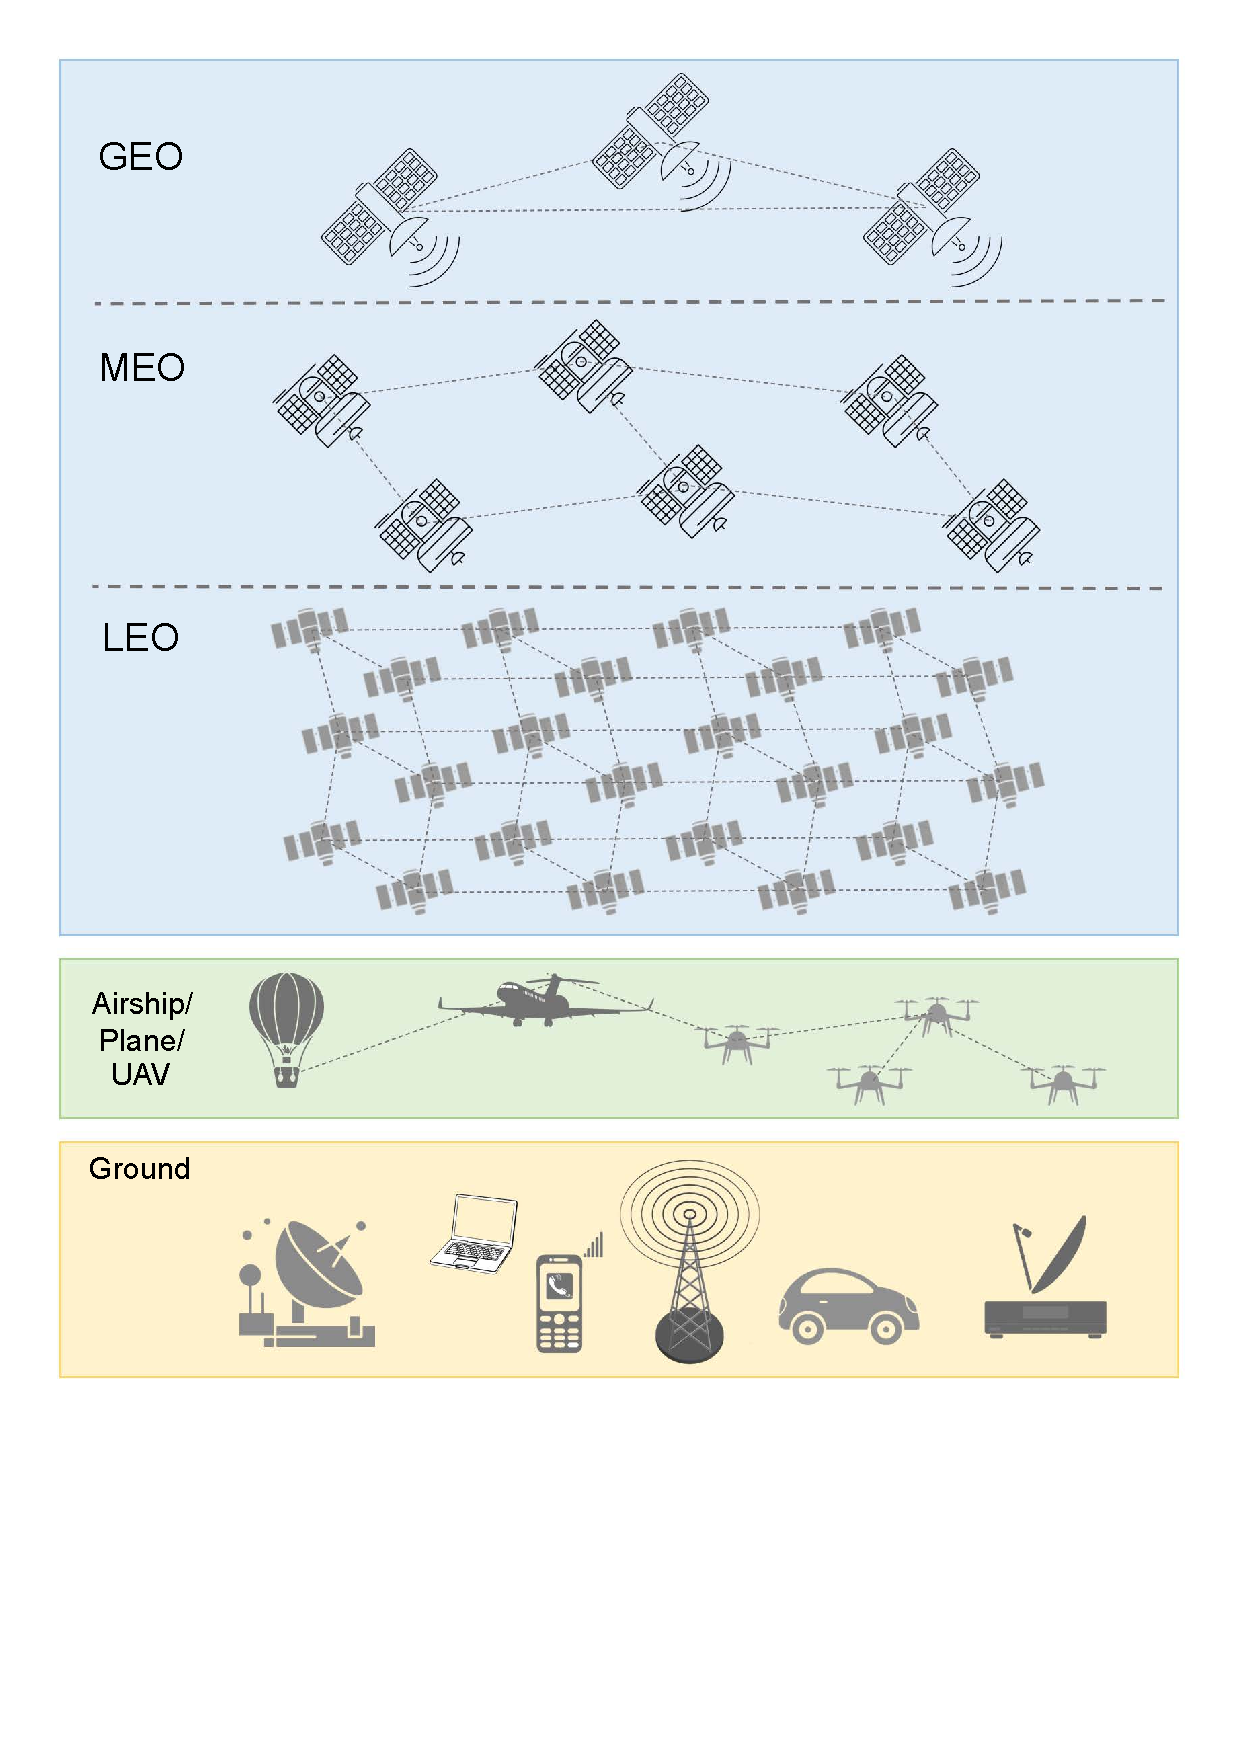
\includegraphics[width = 0.48\textwidth]{fig5.pdf}
  \caption{The architecture of a space-air-ground integrated network consists of three network components that can communicate with one another via radio frequency signals. The space network comprises satellite constellations categorized as GEO, MEO, and LEO. The air-network includes UAVs, airships, and balloons and is an aerial mobile system. The ground network, also known as the terrestrial network, primarily comprises cellular network, mobile ad-hoc network (MANET), and wireless local area network (WLAN).}
  \label{Fig5}
\end{figure}




\subsubsection*{Space-air-ground integrated network}

\begin{figure*}[h!]
  \centering
  
    \subfigure[]{
    \begin{minipage}[t]{0.5\linewidth}
    \centering
    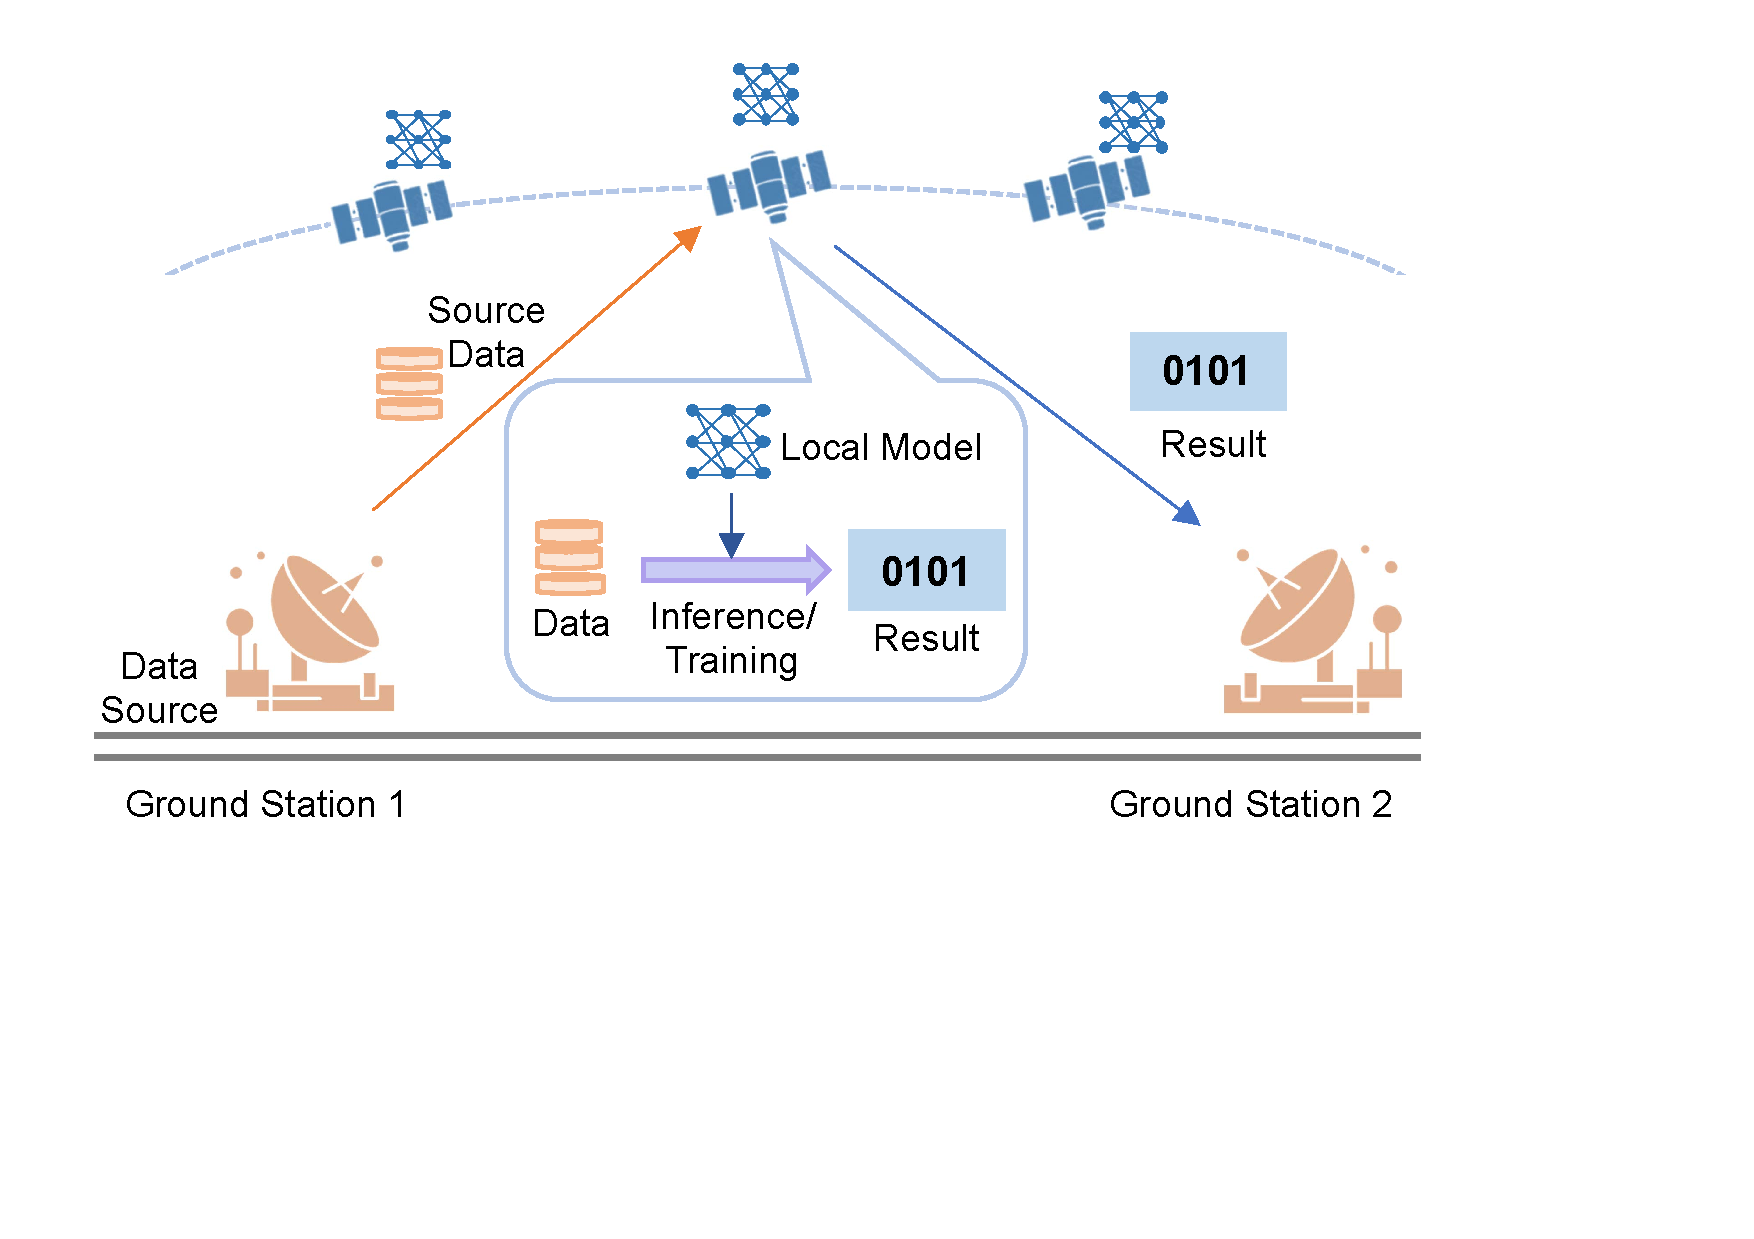
\includegraphics[width=3.6in]{fig8-b.pdf} % 图片路径
    % \caption{fig1}
    \end{minipage}%
    }%
    \subfigure[]{
    \begin{minipage}[t]{0.5\linewidth}
    \centering
    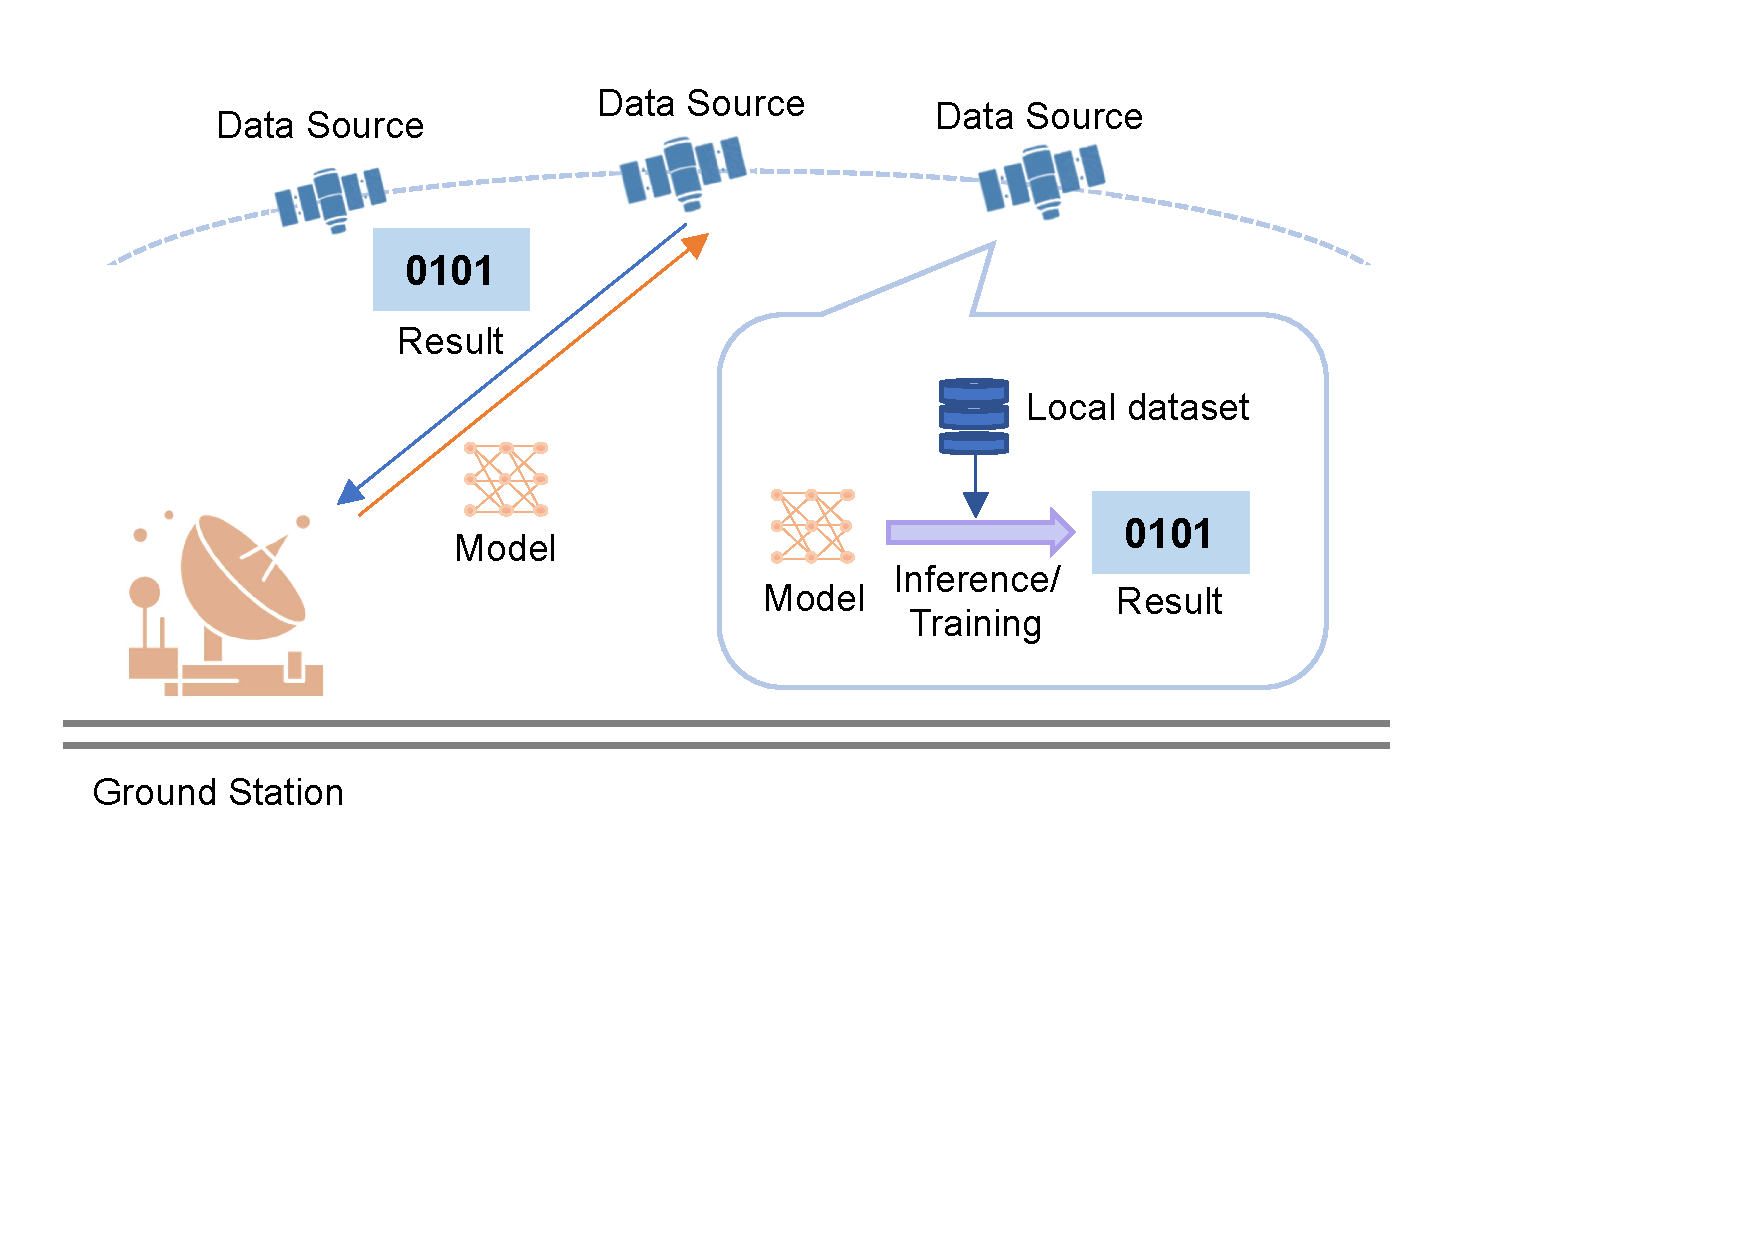
\includegraphics[width=3.6in]{fig8-a.pdf}
    %\caption{fig2}
    \end{minipage}%
    }%

    \centering
    \caption{Satellites accept data from the ground station (a), and process these data by local model independently or jointly, the result will be transmitted to the original or another ground station. For example, satellites offer computation for remote area. Applications as (b) means satellites generate data and process them by assisting with the ground station or other satellites. For example, satellites process remote sensing images to reduce the useless transmission.}
    \label{fig8}
  \end{figure*}

In recent years, researchers have been drawn to SAGIN, a network architecture that interconnects space, air, and ground segments to take advantage of their respective strengths, such as the space network's extensive coverage and the air network's flexibility \cite{RN88}. As illustrated in Fig. \ref{Fig5}, SAGIN consists of three primary segments: space, air, and ground, along with the addition of marine communication network in the SAGSIN \cite{RN207}. Smart satellites, particularly LEO satellites, play a crucial role in SAGSINs by offering irreplaceable services for the IoT \cite{RN208}. Therefore, researchers are concerned with OEC in SAGIN. In the architecture proposed by \cite{RN56}, satellites can be divided into edge and cloud nodes and sliced through software defined Dnetwork or network functions virtualization (SDN)/(NFV) technology.


\section{Systems}
\label{sec3-1}
In this section, we introduce the OEC systems from satellite hardware, satellite software and architecture. First, we introduced the satellite hardware platform that can be used in edge computing applications. Second, we introduced the software and operating systems (OS) of the satellite. Finally, we introduce the architecture of satellite edge computing.

\subsection{Satellite Hardware}
\label{sec2-a}

The space industry is growing at an incredible speed. However, reliability and availability still strongly limit the adoption of new technology on-board satellites because of the harsh universe environment. The satellite needs to face extreme difference in temperature and powerful radiation. The commercial off-the-shelf (COTS) devices with advanced chip manufacturing process such as 7nm are unable to cope with single particle events in the space environment, which is harmless to hardware but it can cause many logical errors in software. Hence, redundancy is one of the solutions that can reduce the impact of single particle events on satellite software. In the Starlink constellation, every satellite has four other satellites as redundancy.

% 这里建议分段,尽量一段讲一个主题
COTS devices have the ability to implement state-of-the-art AI algorithms with low-power consumption \cite{RN229}.  Hence, developing AI technology in satellites has vast potential. $\Phi$-Sat-1, equiped with the Intel Movidius Myriad 2 hardware accelerator, is the first satellite that demonstrates the on-board deep neural network for satellite earth observation. $\Phi$-Sat-1 has demonstrated the robustness of the against ionizing radiation, developing a Cloudscout segmentation neural network, run on Myriad 2, to identify, classify, and eventually discard on-board the cloudy images \cite{RN230}. In the future, more and more COTS devices will be equipped as payload to adapt to satellite intelligence applications, but radiation and thermal control remain challenges in satellite designing.

In a recent study, Xu et al. \cite{RN260} proposed a novel server architecture consisting of massive low-power system-on-chips (SoCs). They conducted a quantitative analysis that demonstrated the server's superiority over conventional servers (Intel CPU, NVIDIA GPU, etc) in three critical in-space computing metrics: energy efficiency, weight, and volume. This work inspired the OEC researchers with a hardware platform that can be applied to OEC and provided guidance for simulating OEC on actual facilities.

\subsection{Satellite Software}
Traditionally, on-board software has been written close to the hardware in assembly language, Ada, C, or C++ \cite{sos1}. The OS provides task and resource management, and application software for providing the mission-specific functionality. The OS we use on computers and mobile devices cannot be directly applied in the satellites because satellites face harsh conditions of space, such as high radiation and extreme temperatures. As a result, satellite OS is required reliability and stability.

The last decade has seen increasing use of Linux in spacecraft on-board software, such as Planet and SpaceX \cite{linux1,linux2}. Howerver, the Linux that applied in spacecraft is different from that we used in personal computer (PC) or embedded device.  SpaceX's Linux is a self-made, deeply customized, distributed operating system, which is not a third-party distribution. It also includes drivers for dedicated hardware, as well as hardware-level security enhancements.
 
In recent years, there has been an increasing utilization of Linux in spacecraft on-board software, including Planet and SpaceX \cite{linux1,linux2}. However, the Linux used in spacecraft differs from that used in personal computers (PCs) or embedded devices. SpaceX has developed a self-made, deeply customized, distributed Linux for its spacecraft, which is not a third-party distribution. Additionally, it includes drivers designed specifically for dedicated hardware, as well as security enhancements at the hardware level.

Additionally, SpaceOS-Tianzhuo is an embedded real-time operating system (OS) developed independently by the China Academy of Space Technology for using in the space field. It includes three generations of products: SpaceOS I, II, and III (Tianzhuo). The first two generations of products have been applied to over 300 spacecraft \cite{spaceos}.


\begin{figure}[htbp!]
  \centering
  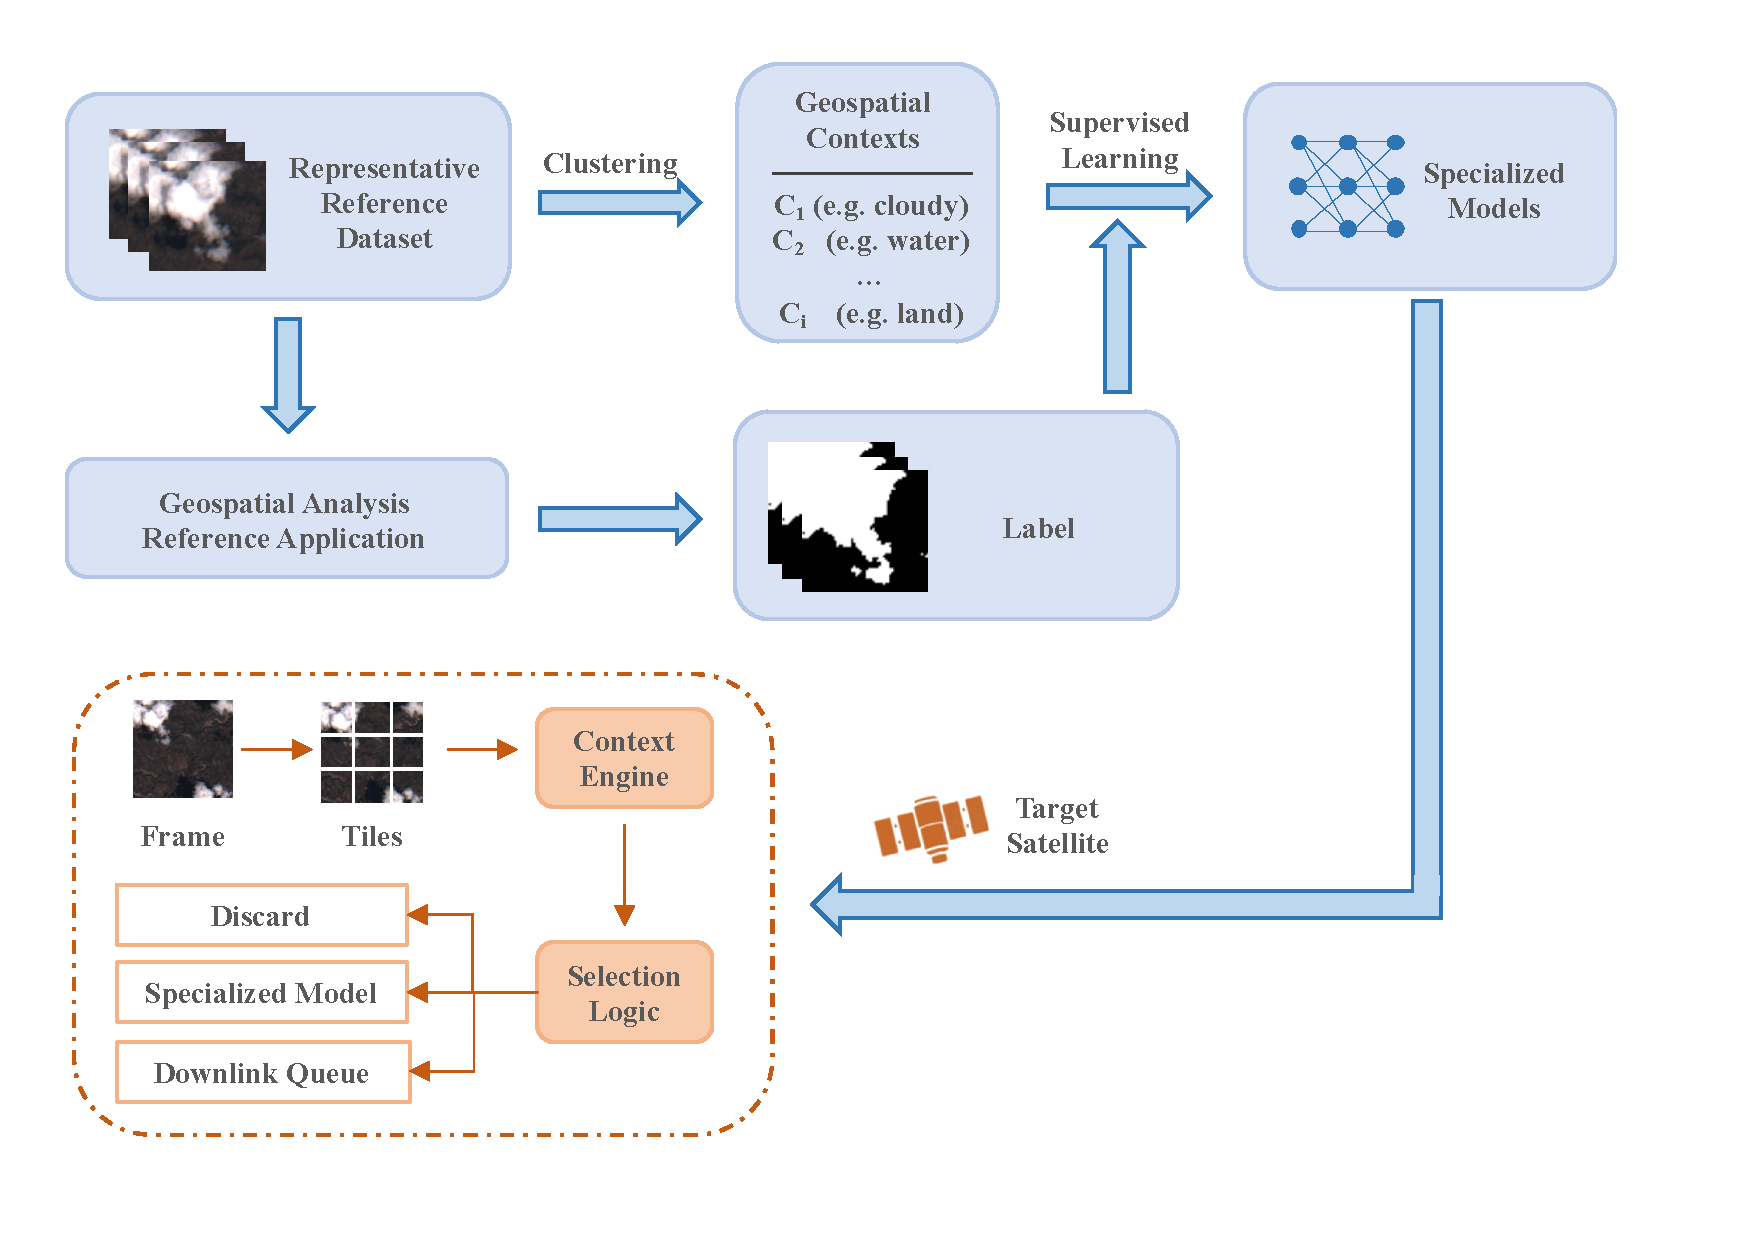
\includegraphics[width=0.45\textwidth]{fig9.pdf}
  \caption{Blue: Before deployment to a target satellite, Kodan clusters the representative dataset into contexts and generates a selection logic. Red: After deployment to a target satellite, Kodan leverages the context engine and the selection logic to meet the soft processing deadline \cite{denby2023kodan}. }
  \label{fig:9}
\end{figure}


\subsection{Architecture}

The design of OEC architecture mainly consider two optimization problems: communication and computation. In terms of communication, the original intention of OEC's design is to reduce the waste of resources caused by satellites transmitting all data indiscriminately under the ``bent pipe" architecture. On this basis, OEC organizes satellite constellations to minimize communication consumption. Nevertheless, the limited satellite computing resources can lead to constraints that cannot be ignored when designing OEC's architecture.

Bradley et al. recently designed an OEC architecture that processed satellite data prior to downlink by identifying the desired signals and only transmitting them. This strategy alleviates the downlink bottleneck \cite{RN57,RN187}. Then, they further proposed an OEC system named ``Kodan" to address the computation bottleneck problem. They designed the selection logic by evaluating the data value of the satellite \cite{denby2023kodan}. As Fig. \ref{fig:9} shows, the architecture design of Kodan considers two parts, one before the development to a satellite, and the other after the development to a satellite. 

Based on representative reference dataset, Kodan deploys specialized models for each target satellite, which exhibits a known execution time on the target satellite hardware as well as known accuracy and precision characteristics across the samples sorted into its context(s) by the context engine. It generates a selection logic before developing to the target satellite by considering its characteristics (computational capabilities, sensor and radio attributes, and orbit parameters) and its ground segment. Then, Kodan leverages the context engine and the selection logic to dynamically select application adjustments for each data sample during the deployment.


\section{Applications}
\label{sec3}
%

\begin{figure}[htpb!]
  \centering
  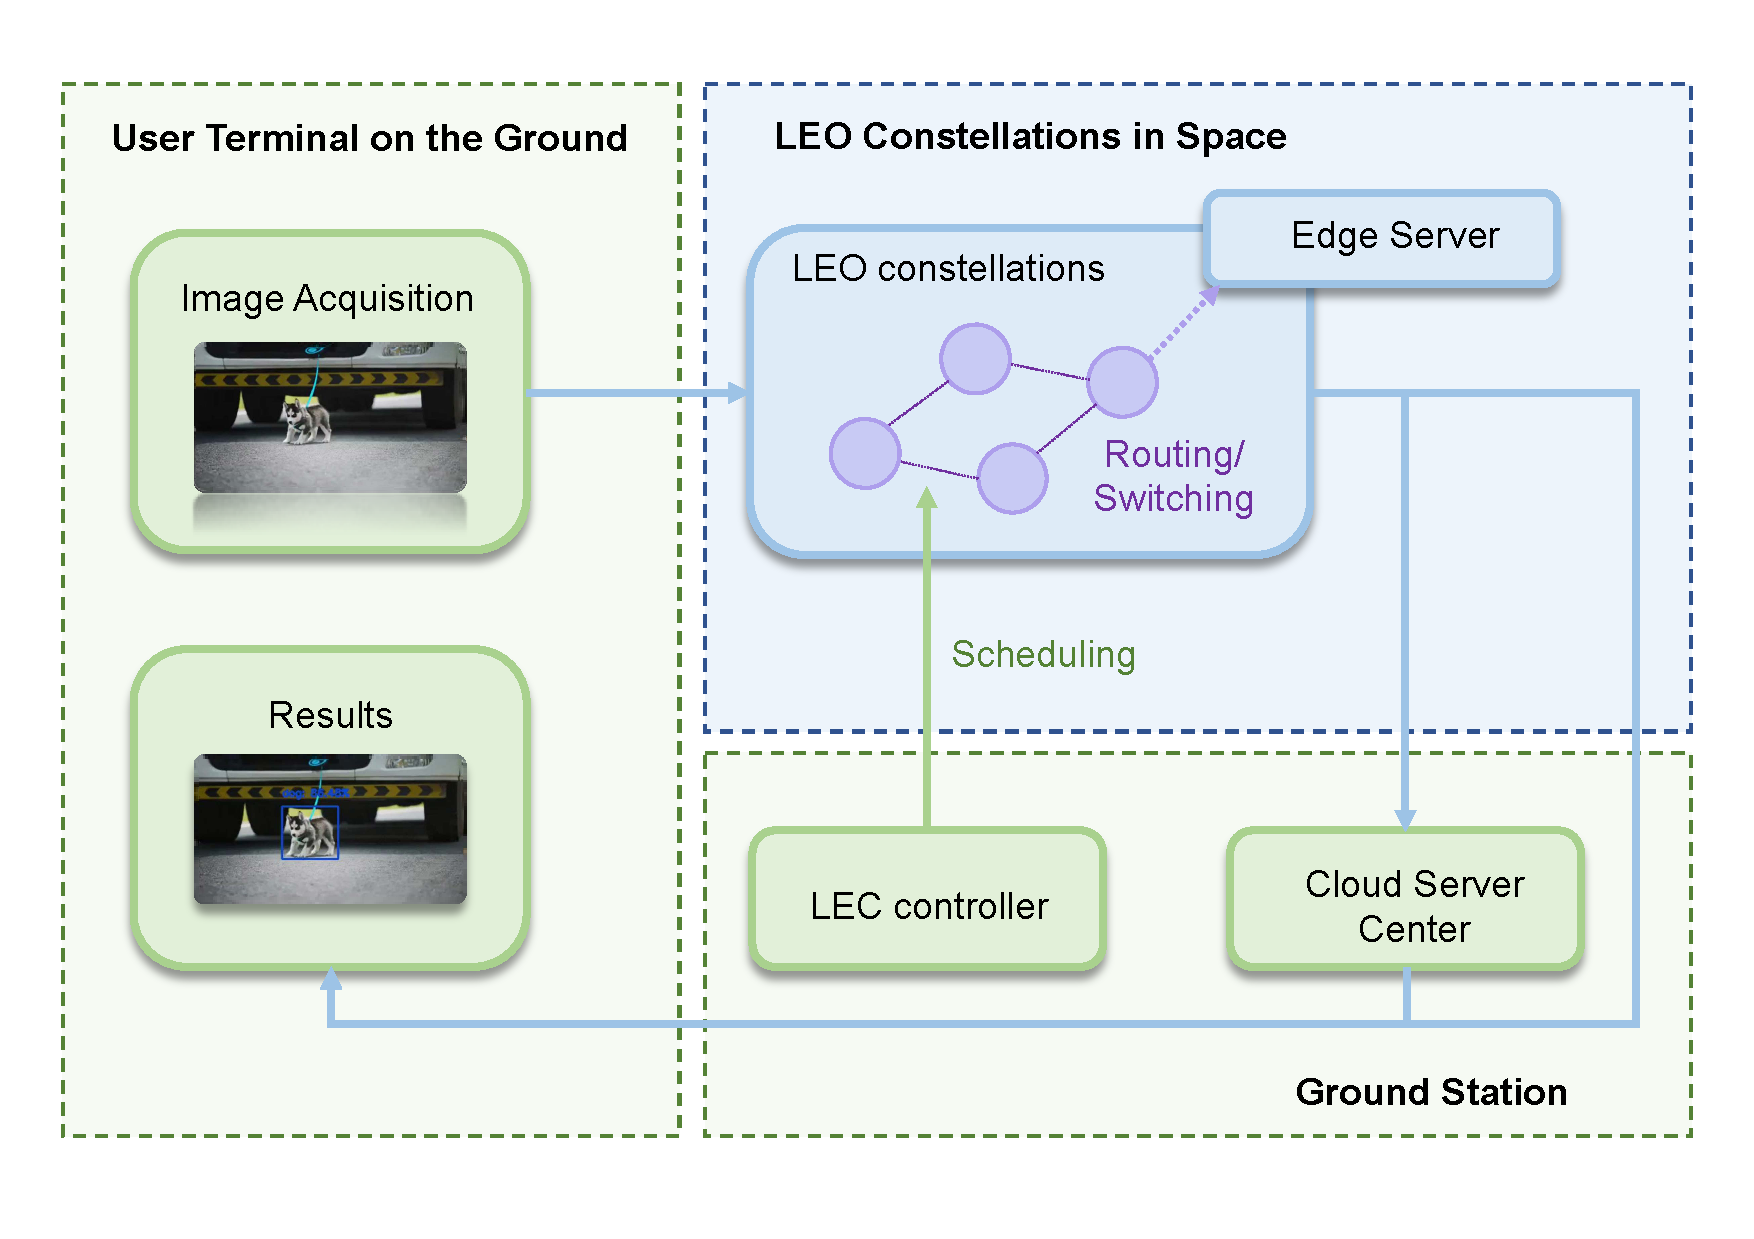
\includegraphics[width = 0.48\textwidth]{fig3.pdf}
  \caption{The framework of object tracking application in OEC \cite{RN55}.} 
  \label{Fig2}
\end{figure}


\begin{figure}[htpb!]
  \centering
  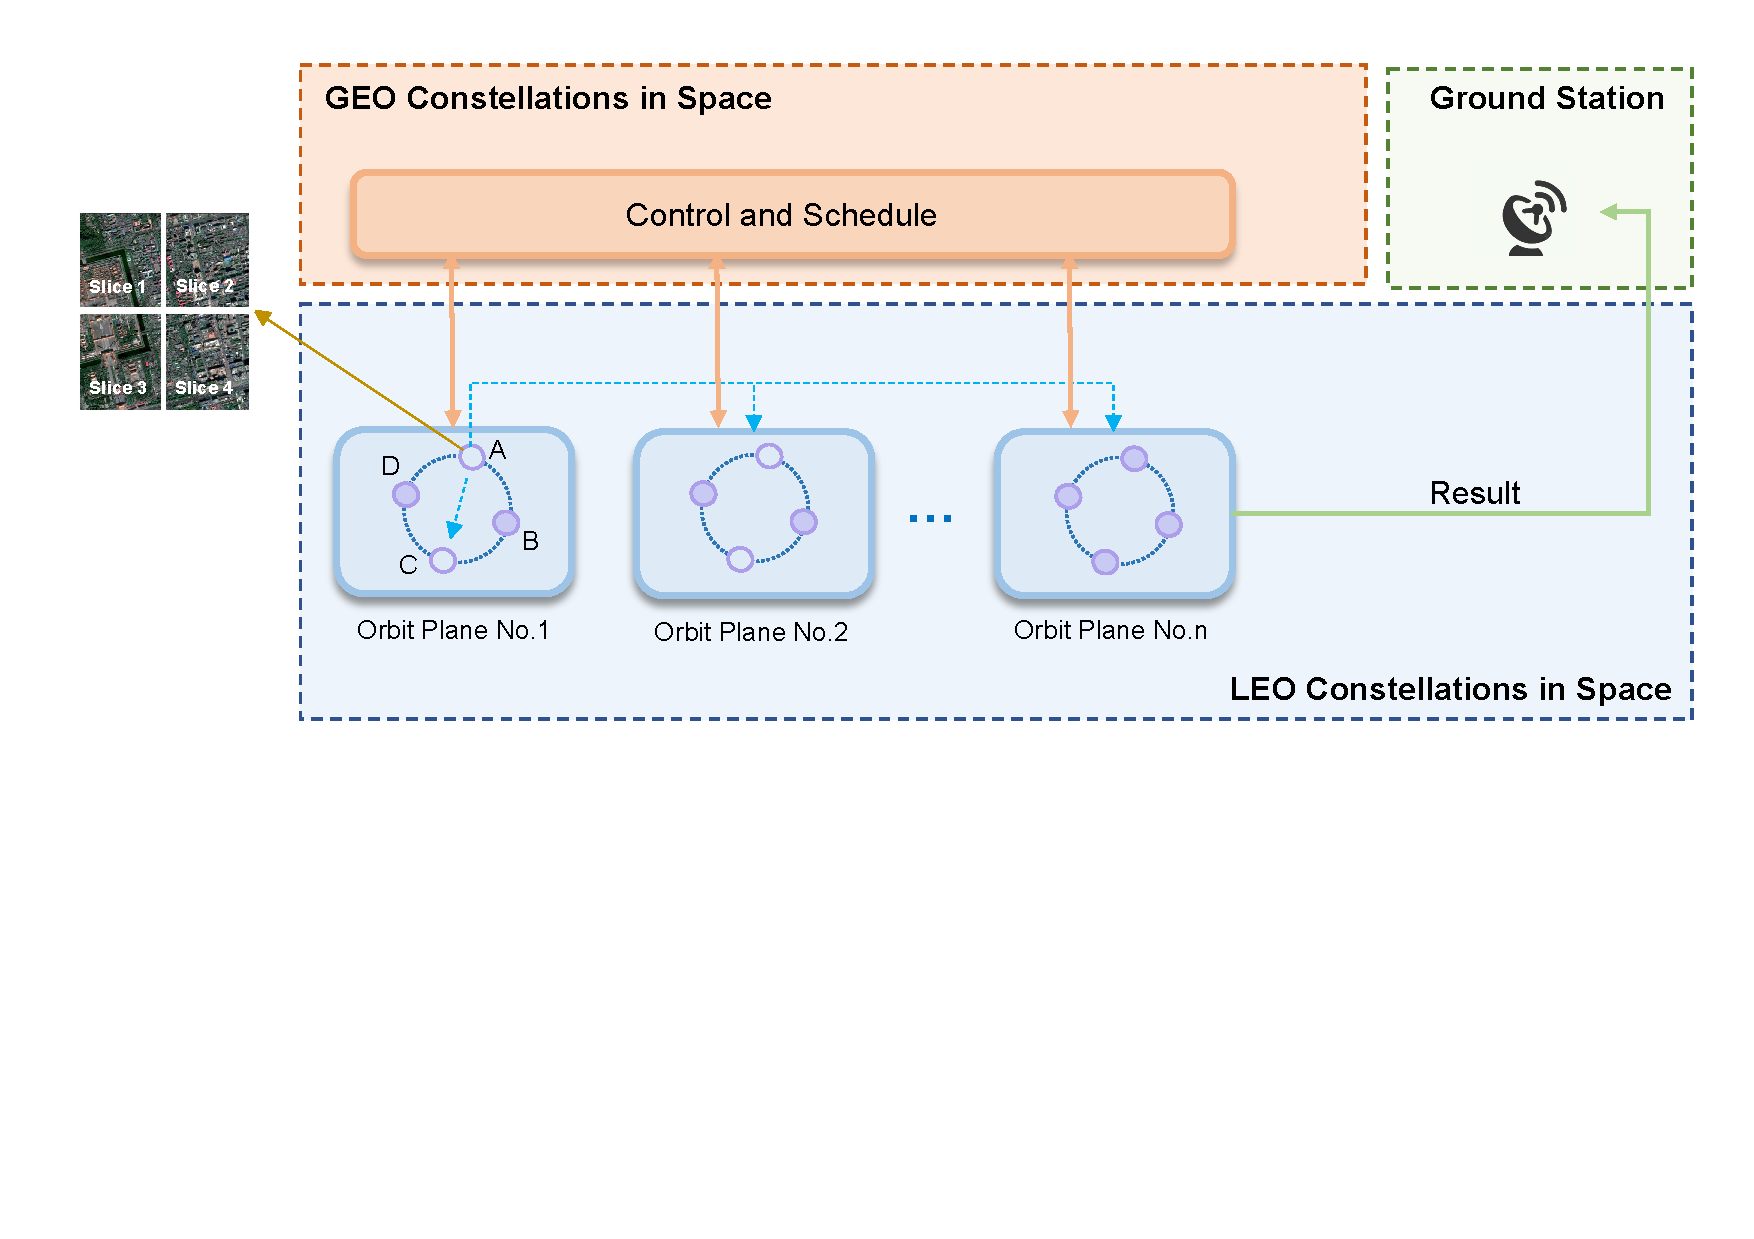
\includegraphics[width = 0.48\textwidth]{fig4.pdf}
  \caption{The framework of disaster surveillance application in OEC.} 
  \label{Fig3}
\end{figure} 


\subsection{Cases of OEC Applications}
% ------------- OEC 应用的案例 --------
An increasing number of emerging applications can benefit from MEC by offloading their computation-intensive tasks to servers located nearby for execution. The potential for utilizing this technology in space is also vast. In this paper, we present two examples to demonstrate the paradigm of OEC. The first example is the object tracking application, shown in Fig. \ref{Fig2}. This application typically consists of three main components: the user terminal, LEO constellation, and ground station. The user terminal submits the computing task to the LEO constellation, and the edge computing LEO (LEC) controller has a global view for task scheduling. Furthermore, the LEC controller can determine whether the task should be offloaded to the cloud \cite{RN55}. When users in remote areas with no terrestrial network access require OEC service, they can request it. Subsequently, the LEC controller selects an appropriate serving LEC node for deploying the service, based on the service discovery process, and the user terminal is informed of which nodes are working for them. Finally, the result is returned.


Fig. \ref{Fig3} shows an example of the orbital computing application, such as disaster surveillance. When satellites are in the same orbit plane, they are referred to as formation flying  \cite{sabol2001} and are relatively static to each other. This implies that they can establish stable communication links all the time, and tasks should be offloaded to satellites in other orbits minimally. For example, when satellite \emph{A} generates a change detection task, it decides whether to offload to another satellite based on its offloading decision algorithm. If offloading, free satellites will be allocated by GEO satellites for use as \emph{A}'s edge computing servers, and \emph{A} will divide the data into several slices and process them according to GEO's guidance. After data processing is completed, the result will be sent to the ground station via optimal routing. Traditionally, remote sensing images are sent to the ground station and processed by terrestrial servers, which include eliminating almost 50\% of useless data. By reducing data transmission volume, orbital computing can lower the pressure of communication. Compared to executing on the ground, execution time has been shown to be almost three times lower \cite{RN46}. In this way, various orbital applications can benefit from OEC by reducing latency and energy consumption.


% 这里根据最后的整体进行修改:
OEC has other practical applications in various scenarios, such as space intelligence, autonomous vehicles, and AR/VR. This section will discuss some of these applications and the benefits of using orbital edge computing in these domains. As shown in Fig. \ref{fig8}, these applications are categorized based on the location of the data source, with satellites serving as training nodes, inference nodes, and relay nodes. We will discuss these applications as the follows.

% 这类应用往往对时延敏感,在远距离的传输过程中,卫星承担边缘计算降低延迟的角色
\subsection{Source data from ground}
As shown in Fig. \ref{fig8} (a), satellites serve as computing or relay nodes to process data received from the ground. Applications in this scenario are highly sensitive to latency. Terrestrial network has unsatisfactory performance in remote transmission due to complex routing, whereas satellite communication offers advantages in terms of coverage and simple routing between remote areas. Satellite edge computing can adapt to applications that require a significant amount of computing resources.

\subsubsection*{AR/VR and UHD video}
Augmented reality (AR) and virtual reality (VR) display exhibit potential to trigger attractive applications, including but not limited to health care, education, engineering design, manufacturing, retail, and entertainment \cite{RN231}, and urtra-high definition (UHD) video can provide better visual differentiation and better depth perception for users \cite{RN233}. However, they face many challenges on complex computation operations, including encoding/decoding and rendering, thus introducing a longer processing time \cite{RN232}. Edge computing provides opportunities for these applications by transfering part of computing pressure to edge device. Howerver, terrestrial networks may fail to provide ubiquitous coverage to surban and rutal areas, and the latency increase obviously with the transmission distance. As an effective solution, OEC  provides ubiquitous access and ultra-long distance with low-latency transmission, opening up further possibilities for these applications \cite{RN81}. 

Celestial \cite{RN102} evaluated the performance of WebRTC video meetings using OEC based on the Starlink network. Three users sent a high-definition video stream with 2.6 Mb/s while receiving video from the others. The experiment showed that the end-to-end latency of both the satellite servers and cloud servers for at least 80\% of the video conference duration was below a maximum round-trip time (RTT) of 16 ms and 46 ms, respectively. This confirms that satellite servers have the potential to significantly improve the quality-of-service (QoS) for clients in latency-sensitive applications.


% 如何进一步介绍,OEC在Ar vr的应用
\subsubsection*{Internet of Vechicles and Autonomous Driving}

The Internet of Vehicles (IoV) comprises a combination of vehicle auxiliary devices and roadside infrastructure that aims to enhance the safety, security, and efficiency of roadway transportation. It also offers different services to various types of vehicles, including private cars, taxis, and buses. Satellites have become a vital element in providing positioning and navigation services for vehicles, and they are an essential component of IoV \cite{RN234}. Yu et al. \cite{RN235} suggest addressing the challenge of providing vehicular networking services in remote or disaster-stricken areas using edge computing and satellite network. Their proposed fine-grained joint offloading and caching scheme leverages the orbit-ground collaboration to provide communication services for vehicles in rural areas, isolated islands, and remote places where terrestrial infrastructure is not available. The scheme aims to provide real-time Enhanced Cellular Satellite Assisted Global Navigation System (EC-SAGINs) services for terrestrial vehicles.

The integration of multiple information, including satellite navigation, road conditions, and traffic flow, among others, enable the implementation of autonomous driving technology, with artificial intelligence (AI) serving a notable role in decision-making processes \cite{RN81}. However, AI-based decision-making requires significant computing resources. Edge computing has emerged as a potential solution, providing lower-latency and greater computing resources for autonomous driving. Satellite edge computing could serve as an auxiliary solution to the inadequate and uneven distribution of ground computing resources. This auxiliary process can provide a more stable and reliable AI decision-making scheme for autonomous driving.

\subsection{Source data from space}
As shown in Fig. \ref{fig8}(b), satellites can serve as a data source and participate in joint training/inference of models through inter-satellite links. Additionally, ground stations can send models or instructions to the satellites. This paradigm offers a significant advantage by avoiding extensive data transmission between satellites and ground stations. As a result, it is beneficial in terms of saving satellite communication costs and improving the intelligent decision-making capabilities of satellites in orbit.

\subsubsection*{Earth observation} 
Satellites are essential for capturing earth data in various fields, such as weather, vegetation and urban development. The data generated is growing rapidly in terms of size and variety, which creates immense pressure on space-ground communication \cite{RN237}. However, OEC can analyze this data, provide near real-time analysis, and significantly enhance decision-making processes. One specific application of this technology is the real-time monitoring of natural disasters. By quickly detecting and transmitting critical information to ground stations, response times can be greatly improved \cite{RN187}. Additionally, satellite edge computing can identify invalid images caused by cloud cover in orbit, which reduces the cost of data transmission to the ground \cite{RN13}. Environmental monitoring is another potential application of satellite edge computing. Tracking changes in land use, forest cover, and ocean temperature provide an opportunity to quickly identify changes and send alerts to stakeholders for timely action. Moreover, multiple agile satellites can utilize satellite edge computing to solve the scheduling problem, enabling on-orbit decision-making and intelligent mission planning \cite{RN236}. These applications demonstrate the potential of satellite edge computing to enhance the efficiency and effectiveness of earth observation missions.

\begin{figure*}[h!]
  \centering
  
    \subfigure[]{
    \begin{minipage}[t]{0.5\linewidth}
    \centering
    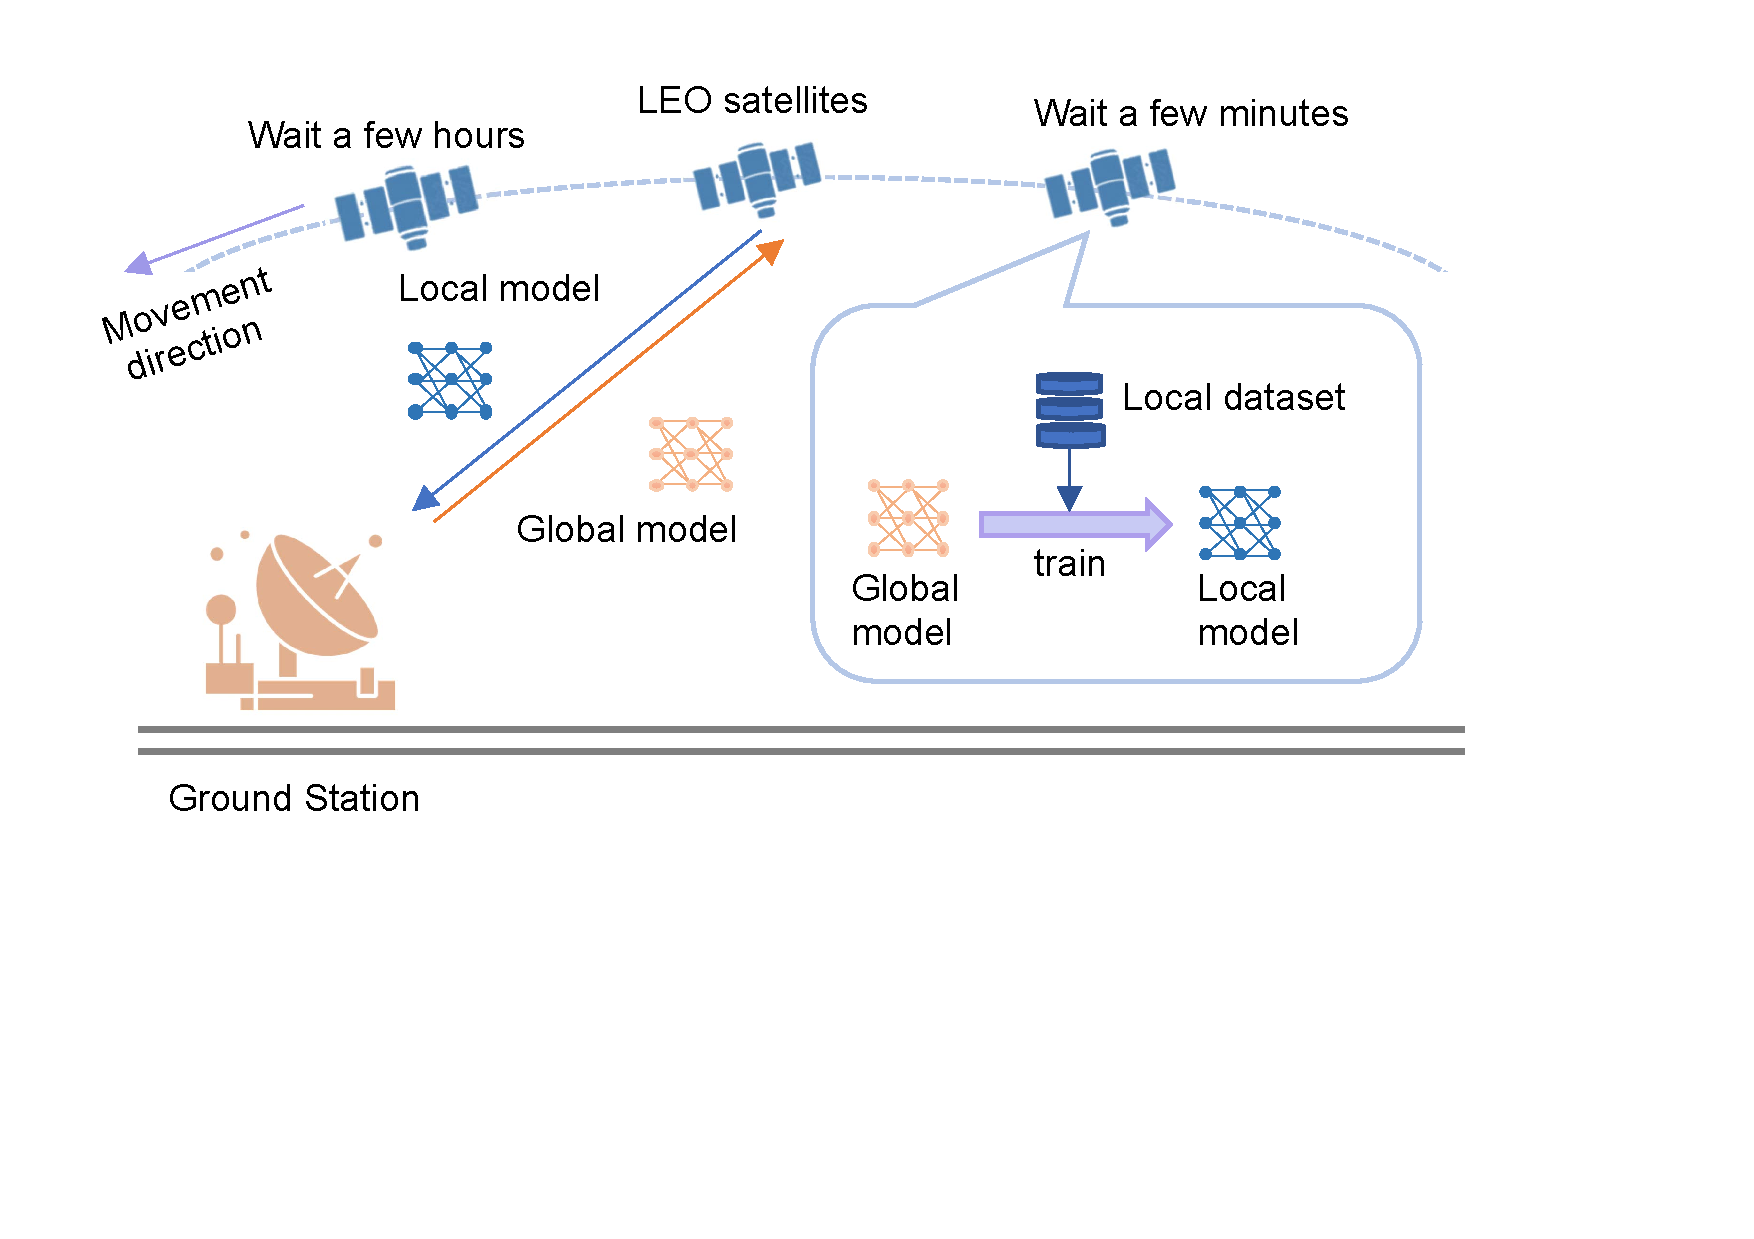
\includegraphics[width=3.6in]{fig6-a.pdf} % 图片路径
    % \caption{fig1}
    \end{minipage}%
    }%
    \subfigure[]{
    \begin{minipage}[t]{0.5\linewidth}
    \centering
    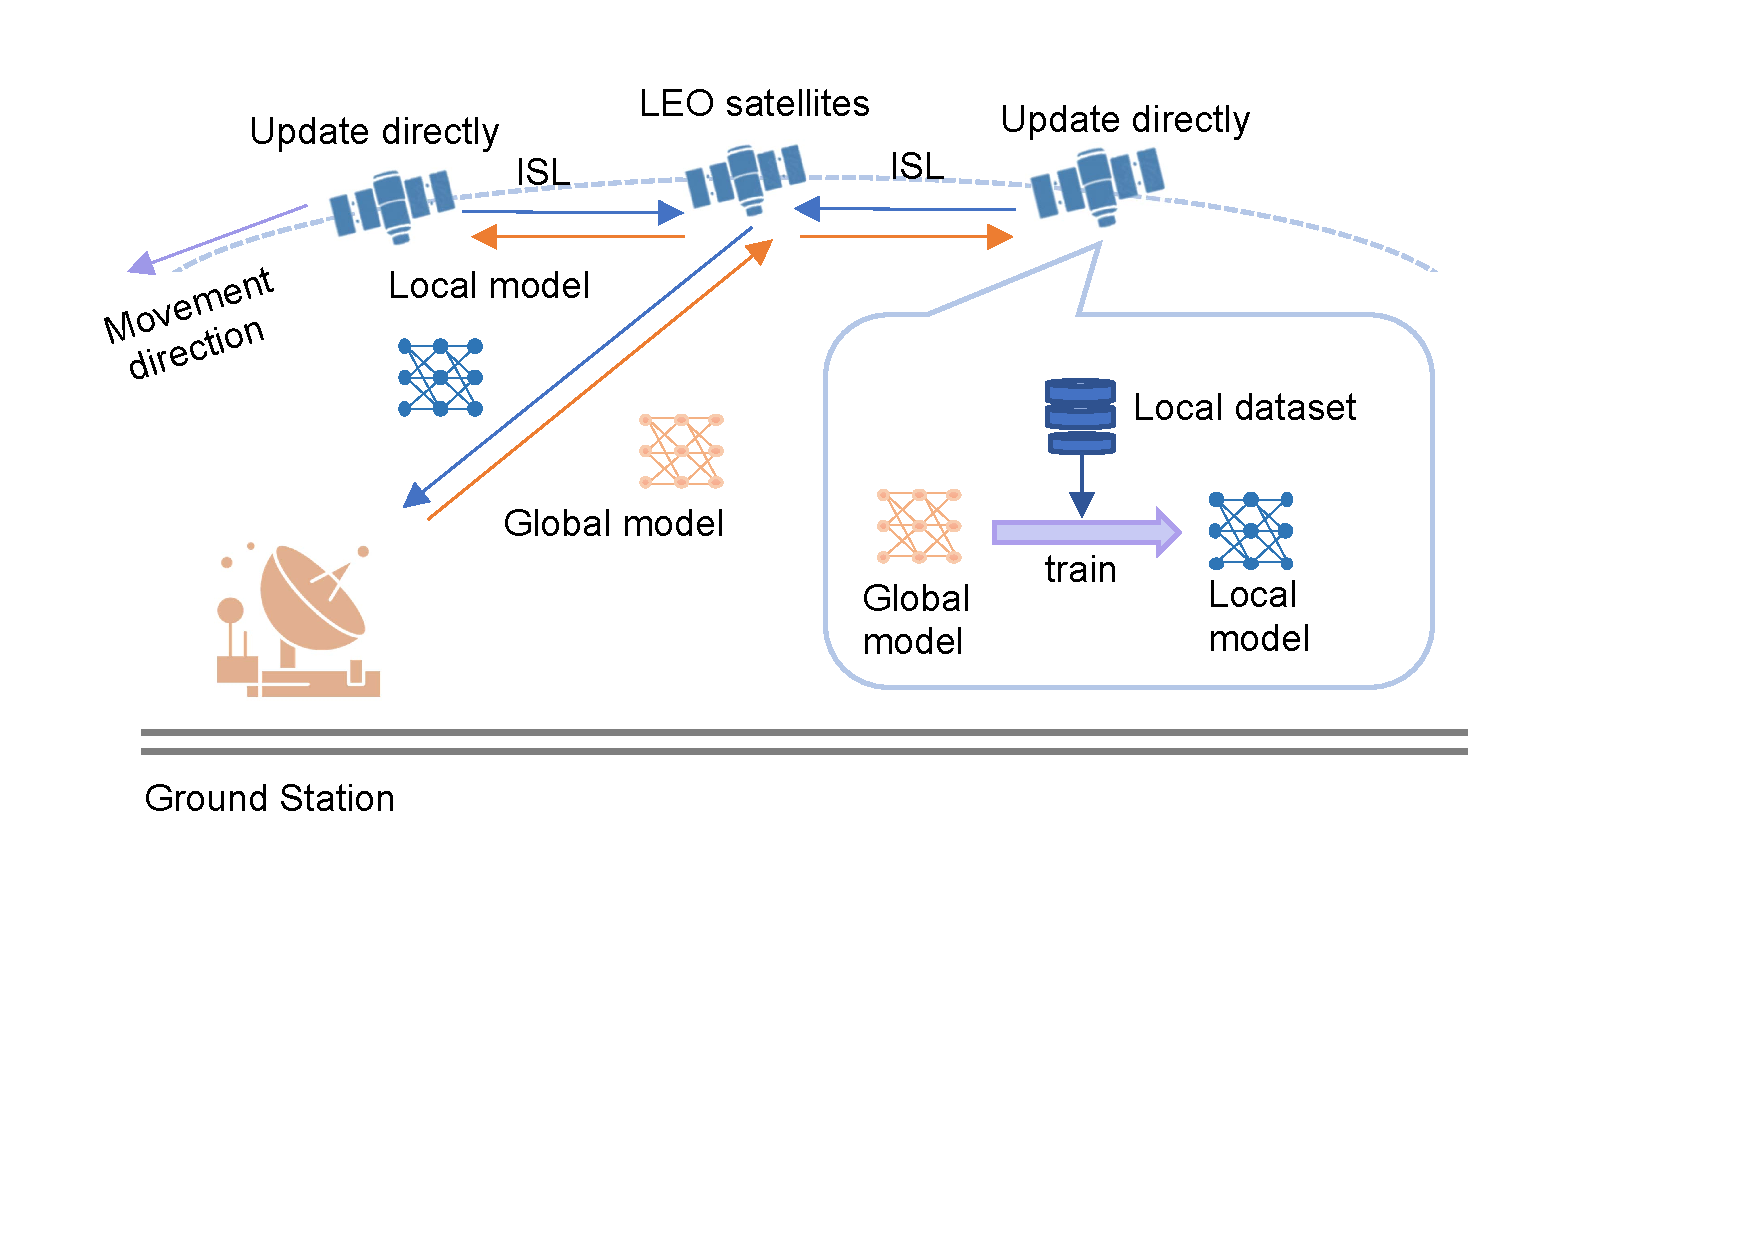
\includegraphics[width=3.6in]{fig6-b.pdf}
    %\caption{fig2}
    \end{minipage}%
    }%
    
    \subfigure[]{
    \begin{minipage}[t]{0.5\linewidth}
    \centering
    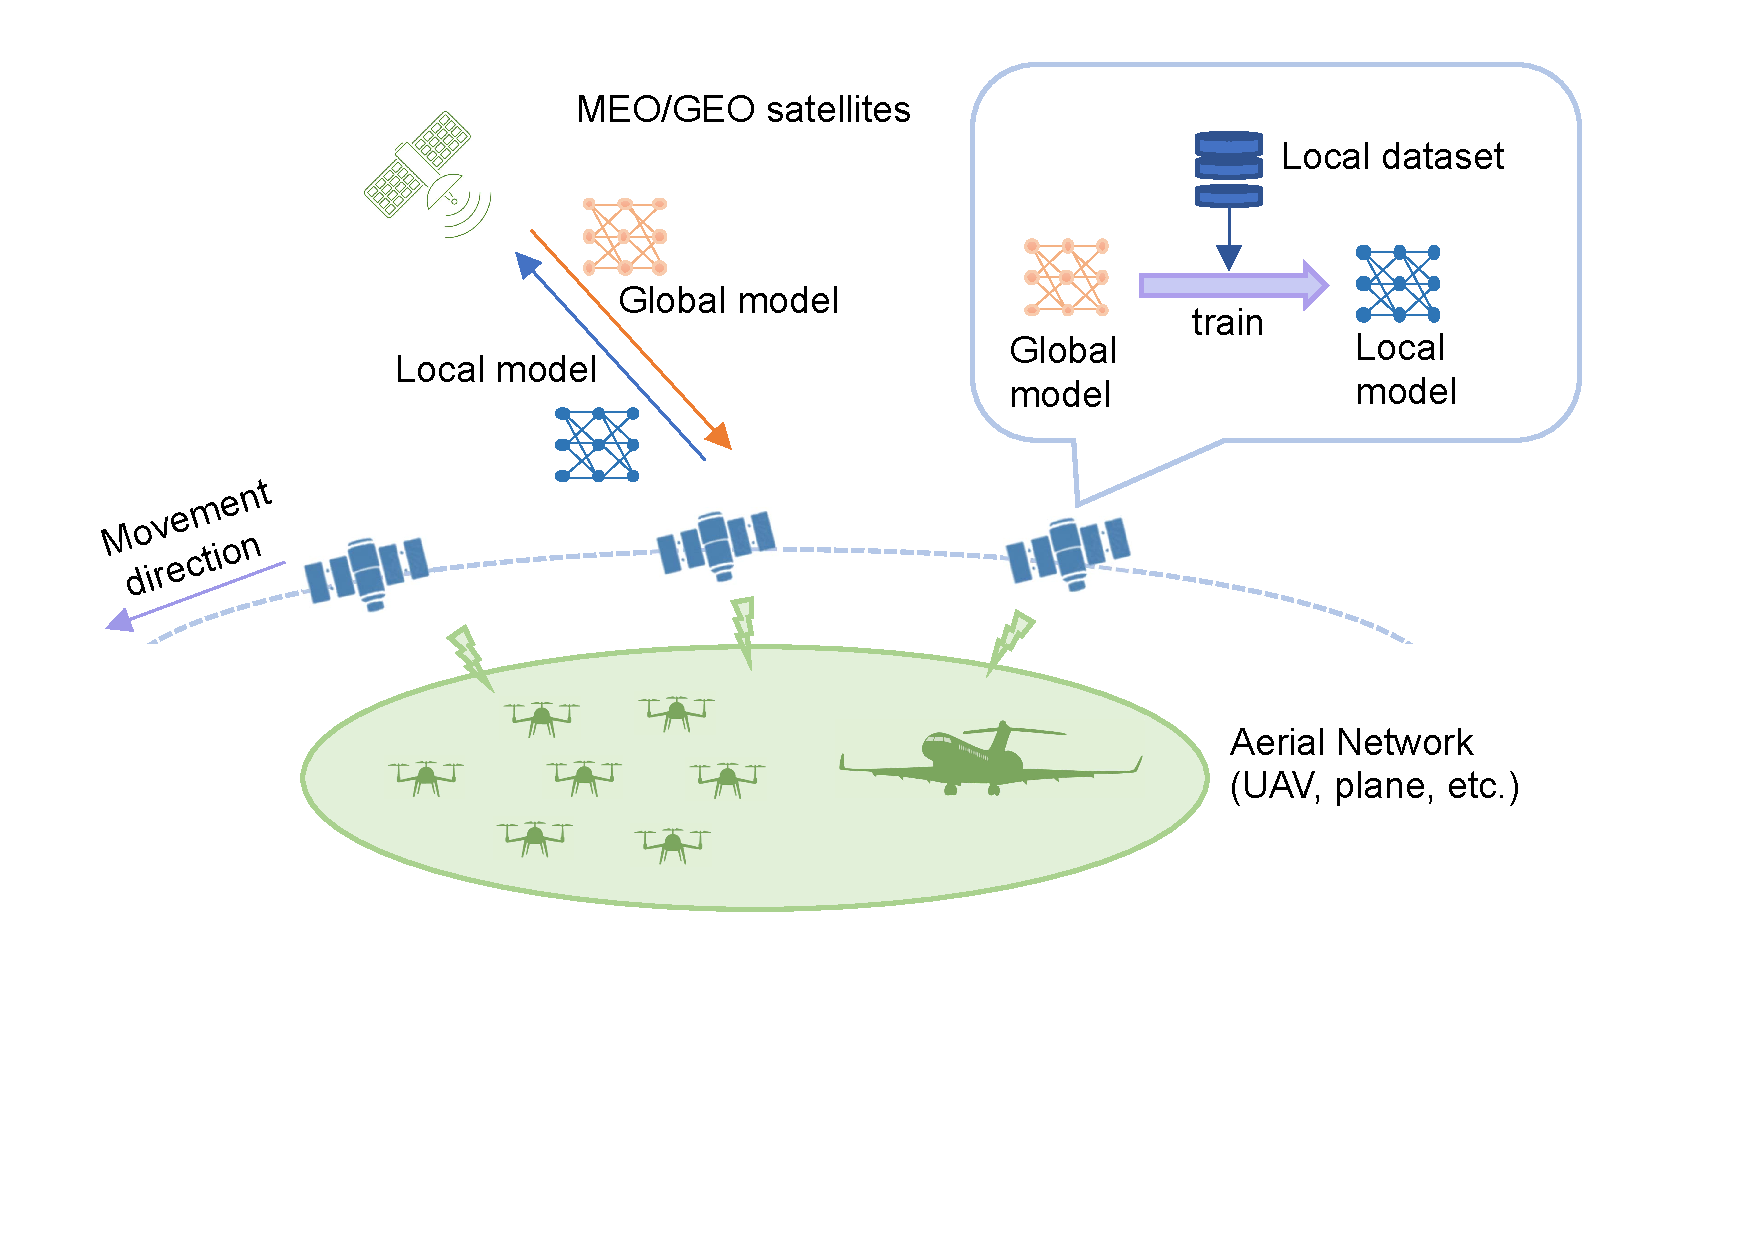
\includegraphics[width=3.6in]{fig6-c.pdf}
    %\caption{fig2}
    \end{minipage}
    }%

    \centering
    \caption{FL without (a) and with (b) ISLs in a satellite-ground system, and (c) is LEO-GEO system. In the case of (a), satellites have to queue until they are within range of the ground station, but in case of (b), satellites linked by ISLs can directly update the model as long as one of them is connected to the ground station. In case of (c), GEO satellites perform a similar role as ground stations, but offer superior coverage and can avail of the advantages of ISLs. \cite{RN217}. }
    \label{fig6}
  \end{figure*}
  

\subsubsection*{Scientific research} Scientific Experiments satellites such as DArk Matter Particle Explorer (DAMPE), Quantum Experiments at Space Scale (QUESS), etc. are used to gather data for scientific research. Scientists obtain a large amount of experimental data from these satellites for space exploration and other missions, which often require transmission via satellite-ground links for subsequent analysis on the ground, a process that is inefficient. Edge computing on satellites, however, seeks to minimize data transmission and even enable in-orbit data analysis and processing.

Several scientific experiment satellites, including the Dark Matter Particle Explorer (DAMPE) and Quantum Experiments at Space Scale (QUESS), are instrumental in gathering data for space exploration and other scientific research missions. Although a considerable amount of experimental data is obtained from these satellites, transmitting the data via satellite-ground links for subsequent analysis on the ground is often an inefficient process. Therefore, OEC can assist scientific satellites in completing on-orbit data processing, reducing unnecessary data transmission.

\subsubsection*{Satellite federated learning}
With the increasing demand for data-driven solutions in various fields, such as agriculture, healthcare, and environmental monitoring, federated learning has emerged as an attractive technique that addresses the challenges associated with centralized data processing and privacy concerns related to traditional machine learning methods. Satellite federated learning is a novel approach that combines the power of satellite technology and machine learning to enable efficient and privacy-preserving data analysis across geographically distributed data sources. For instance, in environmental monitoring, satellite federated learning can analyze multiple sources, such as satellite imagery, ground sensors, and weather stations, to monitor air and water quality, track deforestation, and predict natural disasters. By federating the data and applying machine learning algorithms, accurate models for environmental prediction and monitoring can be developed, while protecting data privacy. In this paper, we summarize three typical architectures of satellite federated learning, as shown in Fig. \ref{fig6}, and discuss their characteristics. Moreover, we provide a comparison of selected articles that may facilitate further study in Table \ref{tab:4}.

Razmi et al. \cite{RN209} proposed using satellite federated learning (FL) based on LEO Mega-Constellation. This technique enables data to stay in the satellite instead of being downloaded to the ground station, saving time and communication energy. The FL-Based Architecture typically consists of two planes: satellite and ground, and Chen et al. \cite{RN225} explored their roles in FL. It shows that using a ground station as the server is more feasible than LEO satellites. However, using LEO satellites as the server results in less delay and faster convergence. Jing et al. \cite{RN214} introduces a new FL architecture that consists of UAV-LEO-MEO. Fig. \ref{fig6}(a) shows the architecture of the GS-LEO without ISLs, which is the basis of most studies \cite{RN209,RN210,RN211}. The most significant drawback of this architecture is the issue with satellite idleness and model staleness because the global model update needs to wait for all of the client satellites to upload their local model.

Fig. \ref{fig6} (b) illustrates the GS-LEO architecture with ISLs. In this architecture, client satellites can update the model directly if at least one of them has a connection to the GS \cite{RN215,RN217}. Specifically, more research has been conducted on intra-orbit ISLs, rather than inter-orbit ISLs because the latter are highly dynamic, making them vulnerable to Doppler shift and requiring more cautious connection planning \cite{RN227}.

LEO satellites have a short duration of visiting a GS, which is typically in the range of tens of minutes. Consequently, Jing et al. \cite{RN214} replace GS with MEO to provide more visit time and reduce transmission delay and energy consumption. Additionally, they utilize high attitude platforms (HAP) and UAVs as an integral part of the server-side. This paradigm is illustrated in Fig. \ref{fig6} (c). Similarly, Cheng et al. \cite{RN81} focuse on a space/aerial-assisted computation offloading algorithm based on unmanned aerial vehicle (UAV)-satellite-ground architecture.

Fig. \ref{fig6}(a) and (b) are summarized as space/ground-assisted architecture, while Fig. \ref{fig6}(c) is categorized as space/aerial-assisted architecture. The former case is suitable for various earth observation applications, including urban planning, disaster management, and climate change mitigation \cite{RN216}. It helps to avoid the transmission of large volumes of data to ground stations. The latter case provides several advantages, including being less expensive, offering better visibility, allowing for better communication, and easy relocation \cite{RN212}. Additionally, it can facilitate edge computing for unmanned aerial vehicles (UAVs) and airplanes. The rest of Fig. \ref{fig6}(c) comprises the LEO-GEO architecture that eliminates the aerial network segment. The LEO-GEO configuration is useful for autonomous mega LEO satellite constellation management \cite{RN217}. Besides, Tang et al. \cite{RN226} introduced the potential advantages and applications of FL in SAGIN. They discussed how FL can assist in solving resource scheduling problems in SAGIN. In summary, all these architectures aim to address the challenge of transmitting huge volumes of data from LEO satellite constellations, which leads to excessive spectrum occupancy.

\begin{table*}[htbp]
  \centering
  \caption{comparison of satellite FL architectures}
  \label{tab:4}
  \begin{tabular}{|c|c|c|c|c|c|c|}
  \hline
  \textbf{Objective} & \textbf{Name} & \textbf{Reference} & \textbf{client} & \textbf{server} & \textbf{Communication} & \textbf{Solution} \\ \hline
  \makecell[l]{LEO satellites generate a huge number\\ of datasets but need to be  transmited to\\ GS, which is inefficient. }& - & \cite{RN209} & LEO & GS  & no ISL & \makecell[l]{They firstly proposed satellite FL, \\ and apply FedAvg \cite{RN224} to show its\\ excellent performance.}   \\ \hline

  \makecell[l]{FL algorithms among satellites and \\ground  stations have challengs in unique\\ trade-off  between staleness and idleness. } & FedSpace  & \cite{RN211} &  LEO & GS & no ISL& \makecell[l]{They presented FedSpace, which \\ considered a heuristic GS update \\procedure and gradient buffering \\ to speed up convergence.}   \\ \hline   

  \makecell[l]{Based on the predictability of \\GS-satellite visiting lengths. The model \\ staleness  can be reduced by designing\\ an  appropriate scheduler.} & -  & \cite{RN219} &  LEO & GS & no ISL & \makecell[l]{They designed a scheduler based \\on the predictability of GS-satellite \\visiting  lengths to reduce the model\\ staleness.}   \\ \hline  

  \makecell[l]{No research talk about the intra-orbit\\ ISLs  in satellite FL.} & -  & \cite{RN215} &  LEO & GS & \makecell[c]{inter-orbit/ \\ intra-orbit ISLs}& \makecell[l]{They offered a comprehensive \\overview of state-of-art in satellite\\ FL and outline several open research\\ directions.}   \\ \hline  

  \multirowcell{2}[0pt][l]{\vspace{-0.1cm} \\ The costs of satellite communication can\\ be saved by FL, but no evaluation about\\ these schemes.}  & \multirowcell{2}{\vspace{0.2cm} \\- } & \multirowcell{2}{\vspace{0.2cm} \\ \cite{RN225}} &  LEO & GS &  \multirowcell{2}[0pt][c]{\vspace{0.2cm} \\ intra-orbit ISLs} & \makecell[l]{They proposed schemes consider \\the preliminary combination of FL \\ and LEO satellite systems. The }   \\ \cline{4-5} 
 & & & GS & LEO & &  \makecell[l]{evaluation indicates that GS-LEO \\ based method has better training\\ performance than LEO-GS.}\\ \hline

  \makecell[l]{No research address the intrinsic \\properties of satellite constellations such\\ as their  non-visibility and predictability \\behavior.} & -  & \cite{RN217} &  LEO & GS/MEO & intra-orbit ISLs& \makecell[l]{They leveraged the predictability of \\satellite movements and partial\\ aggregating to massively reduce the \\ training time and communication\\ costs.}   \\ \hline  

  \makecell[l]{Wireless channels between satellites and\\ GS are highly unpredictable and \\unreliable.} & FedHAP  & \cite{RN212} &  LEO & HAP & \makecell[c]{intra-orbit ISLs, \\satellite-HAP, \\inter-HAP}& \makecell[l]{They introduced high altitude \\platforms into  a synchronous FL \\framework as server, and explore \\inter-satellite and inter-HAP \\collaborations.}   \\ \hline  

  \makecell[l]{Synchronous FL process can take several\\ days to train a single FL model due to \\straggler satellites.} & AsyncFLEO  & \cite{RN210} &  LEO & HAP & \makecell[c]{intra-orbit ISLs, \\satellite-HAP, \\inter-HAP}& \makecell[l]{They exploited the availability of \\synchronous FL without waitting\\ for all satellites and tackle straggler\\ satellites and model staleness.}   \\ \hline  

  \makecell[l]{The recognition of signal modulation in\\ OEC and satellite FL can decrease the\\ communication costs and guarante the \\ data privacy.} & -  & \cite{RN214} & \makecell[c]{UAV/\\HAP/\\LEO} & MEO &  \makecell[c]{UAV-MEO,\\HAP-MEO,\\LEO-MEO}& \makecell[l]{They formulated a joint delay ratio\\ and energy efficiency optimization\\ problem and solved by Q-learning. }   \\ \hline 

\end{tabular}
\end{table*}

  
\section{Simulators and Testbeds} 
% 建议testbed
% \section{Experiment and Simulator}
\label{sec4}

The emergence of cloud computing and edge computing has led to remarkable advancements in multiple algorithms and applications. This progress has also brought about the development of exceptional simulation tools explicitly designed for cloud/edge computing, such as \textit{Edgecloudsim} \cite{RN140}, \textit{iFogSim} \cite{iFogsim}, and \textit{MockFog} \cite{mockfog}. However, as a nascent technology, OEC necessitates a more focused evaluation system and specializes simulation tools. This is because of the distinguished differences between satellite network and ground network. As such, this section compiles comprehensive details on the satellite configurations and simulation tools used in current OEC research. Our expectation is to provide guidance and to serve as a reference for future work in this field. Given the diverse configurations of satellite constellations, the same algorithm may introduce substantial variations when used in different scenarios. Furthermore, we have also summarized the evaluation systems and metrics utilized in relevant studies to provide guidance for the subsequent experimental design in this section. Finally, a testbed for OEC is introduced, which can provide a potential experimental platform for future work in this realm. Nevertheless, such research is still relatively limited in comparison with the abundant edge computing tools used for terrestrial applications. Hence, the testbed can be considered one of the numerous research opportunities in this field.

\subsection{Satellite Constellations for Simulation}
The constellation types used in satellite edge computing are still a topic worth discussing. However, in the face of the challenges of resource allocation and computation offloading in edge computing, some scholars have actively explored possible constellations and conducted simulation experiments. Wang et al. \cite{RN80} established a satellite-terrestrial double edge computing system and simulated a satellite at an altitude of 500km. Additionally, Tang et al. \cite{RN77} studies the computing offloading problem between ground users and satellites based on three low earth orbit satellites, each positioned at an altitude of 784km. To investigate the effects of satellite quantity and orbit altitude on offloading and resource allocation in edge computing, Song et al. \cite{RN76} simulated the algorithm performance of 4 to 6 satellites at orbit altitudes ranging from 500km to 1500km. 

Iridium and Walker are common constellations applied in OEC. A constellation can be defined as $i:t/p/f$, which was previously introduced in Section \ref{sec2-a}. The Iridium constellation, represented by $86.4^\circ:66/6/1$ (780km), consists of 66 low earth orbit satellites evenly distributed in six orbits whose inclination is 86.4 degrees and height is 780 kilometers. Based on the Iridium constellation, Wang \cite{RN4} and Jiang \cite{RN58} conducted research on computation offloading and resource allocation problems, respectively. Similarly, Junyong et al. \cite{RN56} focused on the utilization of edge computing in a satellite-based Internet of Things with a $90^\circ:66/6/1$ (1500km) constellation.  Nasrin Razmi \cite{RN209} proposed satellite federated and conducted simulation experiments based on the $80^\circ:25/5/1$ (500km and 2000km) constellations, and Elmahallawy used an $80^\circ:40/5/1$ (2000km) constellation to study satellite federated learning in two works \cite{RN210,RN212}. Numerous studies have investigated the impact of satellite constellation configuration on algorithm performance, including Tobias' research on the application of edge computing to improve quality of service (QoS) for satellites. In his work, Tobias \cite{RN239,RN105} performed simulation experiments based on four different satellite constellation configurations: Starlink A ($53^\circ:1584/72/1$ at 550km), Starlink B ($81^\circ:375/5/1$ at 1275km), Kuiper A ($51.9^\circ:1156/34/1$ at 630km), and Kuiper B ($33^\circ:784/28/1$ at 630km). Most of the related works are based on LEO satellites, but there are also scholars exploring the possibility of MEO satellites. Taeyeoun \cite{RN60} conducted the analysis of OEC communication performance on the following three satellite configurations: $48^\circ:63/7/1$ (1400km), $48^\circ:190/10/1$ (800km) and $48^\circ:20/4/1$ (20200km). However, the research results indicate that MEO satellites are not a viable option for low latency services due to their long propagation delay.

In summary, LEO satellites are typically deployed at altitudes ranging from 500km to 2000km for edge computing applications, with constellation sizes ranging from dozens to thousands of satellites, depending on the specific application scenario. However, increasing the number of satellites also increases the computational load on simulations, which can quickly consume computing resources. 

% 实验方法和参数
\subsection{Experiment Methods}
Just like edge computing on the ground, experiments on satellite edge computing primarily analyze network, communication, and computational performance. Current works focuse on optimizing resources, computation offloading, and exploring federated learning scenarios in satellite edge computing. This section outlines the familiar experimental techniques and metrics employed in each of these domains.

\subsubsection*{Resource Optimization}
Resource optimization in satellite edge computing aims to minimize latency and energy consumption. As an example, Cui et al. \cite{RN78} simulated a satellite equipped with a CPU capable of 1000 cycles/bit, an energy consumption rate of $3\times 10^{-10}$ J/cycle, and a communication capacity of 10Mbps. Through their experiments, they explore the correlation between a satellite's computational capability and its task execution time. Moreover, \cite{RN80} examines the commercial benefits of utilizing advanced resource allocation algorithms in OEC.

\subsubsection*{Computation Offloading}
Computation offloading is an important strategy for improving the performance and energy efficiency of satellite communication systems. To evaluate the effectiveness of offloading algorithms, researchers often use metrics such as convergence speed, average latency, and energy consumption. For instance, previous work has explored the impact of task quantity and satellite computational ability on latency, and has evaluated the performance of reinforcement learning algorithms in this context \cite{RN18,RN81,RN79}. Other studies have focused on the energy consumption of ground users in scenarios where offloading involves interactions with them \cite{RN77}. By considering factors such as the number of users, the computing and communication capabilities of edge devices, and the types of tasks being offloaded, we can gain insights into the time and energy costs of different offloading strategies.

\subsubsection*{Federated Learning}
In satellite federated learning, algorithms are designed with a focus on convergence rate, accuracy, and the effect of dataset distribution, similar to its ground counterpart \cite{RN211}. Currently, popular datasets used in FL are MNIST and CIFAR-10, so as the satellite FL. Researchers use these datasets to ensure comparability and referenceability in comparing the performance of different algorithms. Moreover, to better meet the requirements set by operational environment characteristics, FMoW \cite{FMOW}, a remote sensing image dataset was utilized by Jinhyun et al. \cite{RN211}. Typical network models employed in satellite federated learning consist of mainstream image classification network such as DenseNet-161 and ResNet-18, as well as simpler neural network like the convolutional neural network (CNN) and multilayer perceptron (MLP).

\subsection{Simulation Tools}
In the field of edge computing, conducting experiments directly on physical infrastructure can pose challenges and expenses, particularly for extensive systems like satellite network. Thus, simulation tools such as virtual network simulators, edge computing simulators and testbeds are crucial for evaluating the performance of edge computing in satellite network. In this subsection,  some popular tools in satellite edge computing experiments are introduced.

\subsubsection*{Satellites Network Simulators} 
The simulation of satellite network plays a pivotal role in the development of edge computing. For instance, the simulation tool, \textit{SNS3} \cite{RN241}, has been developed for this purpose by leveraging the widely used network simulation tool, \textit{NS-3}. \textit{SNS3} is proficient in performing simulation tasks with various satellite link configurations, and analyzing the network at the physical layer. Furthermore, Kssing et al. proposed \textit{Hypatia} \cite{RN242}, which is a network simulation tool specifically designed for simulating large-scale low earth orbit constellations based on \textit{NS-3}. \textit{Hypatia} incorporates unique characteristics of low earth orbit constellations, such as high-velocity orbital motion, to simulate and visualize their network behavior. Likewise, \textit{SILLEO-SCNS} \cite{RN106} concentrates on designing inter-satellite and satellite-ground station network and implements network visualization based on VTK.

\subsubsection*{Testbeds} 
At the time of writing, \textit{Celestial} \cite{RN102} is currently the only testbed available for satellite edge computing. \textit{Celestial} uses the \textit{SILLEO-SCNS} network simulator to accomplish network simulation tasks for large-scale low earth orbit constellations, while carrying out edge computing simulation based on microVMs. One unique aspect of the testbed is its ability to execute a high-definition video conference task based on the Starlink satellite constellation, with servers deployed across South Africa, Cameroon, Nigeria, and Ghana. The results show that OEC effectively lowers the latency in the meeting. \textit{Celestial} also provides support for simulation related to OEC challenges, such as resource allocation, computation offloading, and satellite routing.

% ============================= Ⅳ OEC的关键技术(计算卸载,资源管理) ==========================
\section{Algorithms}
\label{sec5}
There are numerous critical optimization problems in OEC, including computation offloading, resource management, and mobility management. Many of these problems are non-convex, which has stimulated scholars to design an array of optimization algorithms to enhance OEC's efficiency. This section will introduce some of these algorithms.

\subsection{Computation Offloading}
Computation offloading in OEC is the process of transferring computation-intensive tasks or data from a local device with low computation abilities, such as smart mobile devices, to satellites with more powerful computing resources in order to reduce latency and energy consumption. Researchers typically model the decision problem of computation offloading as a mixed integer nonlinear programming problem, which is non-convex and NP-hard. Therefore, deep reinforcement learning-based methods have been widely applied to solve such problems, and have shown promising results \cite{RN18, RN79}. Typically, this problem is modeled as a Markov Decision Process (MDP) and Deep Q-network (DQN) is used to obtain the optimal solution \cite{RN78}. The design of the reinforcement learning process involves four essential components: the environment, action, state, and reward. The agent takes an action based on the current environment to update its state, and evaluates the goodness of its action. The reward given to the agent indicates whether the action is correct or not. A negative reward serves as a punishment, indicating that the agent's action did not meet the required goal. After multiple iterations, the agent learns how to take effective actions based on different environments. In the scenario of satellite computation offloading, the satellite, as an agent, models its communication and computing resources as the environment, while its offloading strategies are modeled as the action space. The task's delay and energy consumption are considered as the state, and the reward function is designed to encourage the satellite to minimize the overall delay and energy consumption of the task. With this design, the satellite can intelligently offload computation tasks to other edge devices after thousands of iterations.

Non-convex problems generally can only be solved using approximation algorithms. Tang et al. \cite{RN77} converted the problems to linear programming and solved them by applying relaxation on binary variables. Additionally, they reduced the computational complexity by implementing the alternating direction method of multipliers to approximate the optimal solution.

In collaborative satellite-terrestrial network, which is a multi-user scenario, can be modeled as a game problem, and Wang et al. \cite{RN4} proved the existence of a Nash equilibrium for these problems and proposed an iterative algorithm to find it. In this model, each device will selfishly choose the strategy that will minimize its own cost. Using queuing theory, the response time and energy consumption of a task can be computed, which are important metrics for optimizing performance. 

\subsection{Resource Managemt}
Increasing satellite computing power may reduce system latency, but may result in higher energy consumption. The optimization of computing and energy consumption can be formulated as a mixed-integer programming (MIP) problem. The optimal solution can be achieved using the Lagrange multiplier method \cite{RN18, RN78}. Wang et al. \cite{RN80} modeled the optimization problem as a mixed-integer nonlinear programming problem and addressed it by Lagrange dual method. Previous studies have attempted to use game theory to optimize ground MEC resource management \cite{RN245}. However, there is relevant no work attempting to use game theory to address the resource management problem in OEC. The above work optimizes resource allocation from the perspectives of the game between task energy consumption and system latency. 
Tobias et al. allocated resources based on satellite selection mechanism \cite{RN239}. They modeled LEO satellite network as 2D tori, and framed the selection of satellites for server placement as a distance-$d$ resource placement problem while considering the QoS constrains.

Optimizing resources such as link delay, bandwidth, and connection time is essential from a communication perspective. Du et al. \cite{RN248} analyzed the cooperative mechanisms of relay satellites in GEO and LEO satellites, and suggested a strategy for multiple accesses and resource allocation in GEO relay for LEO satellite network. Kodheli et al. \cite{RN249} proposed an approach for allocating resources to decrease high differential Doppler values that fall below the standard's maximum limit. Qiu et al. \cite{RN247} suggested a software-defined model that could manage and orchestrate networking, caching, and computing resources in LEO network, thus optimizing resource allocation for the delay and Doppler phenomenon in communication via deep Q-learning. In satellite network utilizing software-defined network and software virtualization technologies, cooperation among resources is feasible. Sheng et al. \cite{RN250} explained the evolution of the multi-dimensional graph model and suggested an optimal resource allocation strategy to enable efficient resource cooperation. Wang et al. \cite{RN246} suggested a dynamic resource scheduling algorithm that employed advanced K-means and breadth-first-search-based spanning tree algorithms (BFST) to manage resources in satellite network.

\subsection{Mobility Managemt}
In the context of OEC, mobility management ensures the service continuity of ground users or satellites and edge equipment, according to the edge satellite's location information, security and network topology. Edge clients in terrestrial mobile edge computing often exhibit random mobility patterns, while satellites fly in fixed orbits with predictable trajectories. This predictability enables the server to receive predefined mobility models, such as the flight trajectory of LEO satellites \cite{RN243}. Zhu et al. \cite{RN79} proposed real-time decision making to assign tasks to satellites based on the channel condition, thus simplifying the mobile prediction process. Li et al. \cite{RN55} designed a LEC controller that developed on the ground. It has a global view - all links' latency and bandwidth, constellation topology and all the satellites' available resources. By this way, the controller can know the movement information of each satellite and make computing decisions by these global information. Carlos et al. \cite{RN240} proposed a control framework for managing large-scale satellite constellations. By using the contact topology information, this framework can design a global flight plan that solves a specific task for a certain scenario based on genetic algorithm. 

Mobility management in a space-air-ground integrated network is more complex as it must consider node mobility across all segments of the network, unlike a single segment of a satellite or terrestrial system. An efficient and seamless ubiquitous communication can be established by using the Hata model in terrestrial systems and the statistical shadowing model in satellite links \cite{RN244}. This provides an example of mobility management from a communciation view. 

% ============================= Ⅵ OEC的问题,挑战和关键技术 =================================
\section{Issue, Challenges and Future Research Directions}
\label{sec6}

% 可以提一下现在的实验平台以仿真为主,可能没法反映真实情况?而构建一个真实的实验平台又成本很高
\subsection{Issues and Challenges}
The vision of a reliable and accessible orbital edge computing service comes with numerous challenges and issues that need to be addressed:

\subsubsection*{Resource-constrained Satellite Payload} Traditional satellite payloads are typically tailored to specific missions, resulting in platform and system incompatibilities when implementing edge computing. Furthermore, updating these payloads' systems and functions poses a challenge. Solar power serves as the primary source of energy for satellites, and proper energy management is necessary given the variance in light exposure and duration. To reduce mission failure rates, satellite energy management must not only minimize consumption, but also consider whether the remaining energy can support mission completion. Additionally, the complex space environment presents challenges for chip fabrication and heat dissipation, both of which impact satellite computing performance.


\subsubsection*{Large-scale Satellite Network} Recently, large-scale low orbit satellite constellations have become a prominent trend in intelligent satellite network. The massive scale of satellite network presents challenges to optimization algorithms. As mentioned earlier, typical NP-hard optimization problems exhibit exponential growth in solution complexity as the number of nodes increases, presenting significant challenges for optimization algorithms in large network. Furthermore, mobility management costs increase significantly within these large-scale network. Using one or a few ground stations to manage the trajectory information of all nodes is no longer practical.


\subsubsection*{Unfavorable Satellite Status} In recent years, all work related to OEC assumes that all the nodes of the satellite are idle and available, but this is a simplification of actual application scenarios, which may be much more complex. Firstly, satellite computing power is varied, and resource distribution is unbalanced. Secondly, the possibility of satellite malfunctions or other factors leading to nodes going offline complicates computations. Finally, in actual applications, a satellite network undertakes diverse services, meaning not all accessible satellites can participate in any given task. Therefore, future research should approach computation offloading and experiments in a manner that accounts for these complexities.

% 不理想的仿真器
\subsubsection*{Non-ideal Simulators} At present, research on OEC is restricted to ground simulation that might not represent the space environment's actual scenario. The mission of ``TianSuan" series satellites \cite{RN13} is to create a computing platform in space, providing an opportunity for OEC researchers. Nevertheless, performing experiments on actual satellite equipment continues to be expensive. Moreover, achieving OEC under the envisioned ``large-scale constellation" seems like a distant undertaking.


% ++++++++++++++++++++++++ 润色分割线 以下内容尚未润色++++++++++++++++++++++++++
% 可以再加上以下内容:
% 1. 卫星硬件的需求,相比地面硬件,需要满足更多的要求,包括重量、体积、功耗等;
% 2. 卫星AI,有更加轻量化的需求,而且星上的遥感AI任务和传统的地面AI场景有较大区别,包括对图片的分割等,有较大的design space,参考brandon lucia今年的ASPLOS论文


\subsection{Opportunities and Future Research}
OEC has a highly anticipated application prospect, which is a trend for satellite network to become more intelligent. There are numerous opportunities for researchers who seek to contribute to its continued development.

\subsubsection*{Software-defined satellite}
The utilization of software defined satellite technology represents a significant advancement in satellite technology. This technology allows for the installation of plug-and-play payloads, as well as the ability to load software on demand. Additionally, satellite functions can be conveniently redefined through software updates to adapt flexibly to various tasks and user needs. Furthermore, this suggests that future satellite network will evolve towards a software-defined architecture. Within this context, satellite resource management by OEC will become even more flexible.

\subsubsection*{Inter-satellite laser link}
In recent years, free-space optical communication has garnered significant interest as it greatly enhances the communication efficiency of satellite network. These types of satellites provide higher bandwidth and lower latency through laser link communication, making them suitable for scenarios which require high communication needs like large-scale satellite distributed computing and collaborative tasks that demand prompt response times.

% 独特的卫星载荷 与地面设施不同,卫星载荷的硬件需要面对极大的温差、极强的辐射。除此之外,卫星的载荷对体积和重量有着苛刻的要求,因为这决定了卫星制造和发射的成本。 应对日益增长的卫星算力需求,研究和开发高效可用的卫星载荷迫在眉睫。
\subsubsection*{Satellite hardware} Unlike ground facilities, satellite payloads' hardware must withstand extreme temperature fluctuations and strong radiation. In addition, volume, weight, mass and mass are subject to strict requirements since they ultimately determine the cost of manufacturing and launching a satellite. With the growing demand for computing power, it is imperative to study and develop efficient hardware for satellite payloads.

% 卫星AI
% 星上的遥感AI任务和传统的地面AI场景有较大区别,遥感数据的价值是不均等的,这意味着遥感图像的预处理可以节约的算力资源和通信资源。Bradley 提出了Kodan,这是一个可以最大化数据价值的系统。通过区分高价值的数据和低价值的数据,使用context-specific model来最大化数据价值。
\subsubsection*{Special AI in space} Due to the aforementioned limitations on satellite hardware, there is a particular need for lightweight AI models in satellites. The design of such models should consider task types, data, and communication resources required for OEC. Additionally, AI tasks in remote sensing differ significantly from those on the ground. Satellite data is sampled without identification, meaning some observations are of high-value to an application while others are of low-value. The OEC system Kodan, which overcomes computational bottlenecks by maximizing data value density \cite{denby2023kodan}, inspired us to explore the design space of data selection in remote sensing tasks.


\subsubsection*{Efficient resource management algorithm}
Resource optimization is a popular research topic in terrestrial network. Satellites have more constraints compared to terrestrial equipment. As a result, researchers are encouraged to investigate advanced and practical optimization algorithms. Existing research uses deep reinforcement learning to solve these problems, but no related work has experimented on larger constellations. Increasing the number of nodes may hinder further applications due to the parameter and convergence speed limitations of deep reinforcement learning network. Therefore, it is imperative to conduct experiments on larger satellite network to align with future practical industrial development trends, requiring better performing optimization algorithms.

\subsubsection*{Diverse business requirements}
The use of intelligent satellite network is being actively explored for potential application services,  including advanced business needs on the ground, such as AR/VR, UHD vedio. OEC offers remote areas the possibility to apply these services. In addition, OEC breaks the inefficient ``bent-pipe" architecture, where satellites collect data and then transmit it to the ground for processing. OEC provides the possibility for autonomous processing for satellites, which saves satellite-ground communication costs and improves mission execution efficiency. In the future, when large-scale LEO satellites are commercialized, satellites can access computing power services for ground users. Furthermore, the application of satellite federated learning can support satellites to update AI models autonomously. Users can implement online update of the model according to their needs. 


\subsubsection*{Testbed}
% 看一下测试床那篇文章进行一下补充
At present, OEC is still a concept, and only one comprehensive testbed work on OEC has been proposed \cite{RN102}. However, due to the large number of nodes in satellite constellations and the complex network topology, developing OEC models on real devices are not feasible. Hence, with the diversification of application scenarios and the introduction of new algorithms, there is an urgent need to develop the more testbeds and improve their performance. To achieve a test-friendly OEC testbed model, it should have the following characteristics:
\begin{itemize}
  \item Accurate satellite constellation simulation. Satellite network topology and satellite mobility models are one of the most important features of OEC tasks. Accurate satellite constellation simulation can realistically simulate the movement of nodes in space. Typically, it can support professional satellite simulation tools such as STK, or develop independent satellite constellation simulation tools. 
  \item Excellent platform compatibility. The testbed should be deployable on actual physical devices to achieve a more realistic simulation. Therefore, the testbed needs to be compatible with various platforms, such as personal computers and various embedded devices.
  \item Customizable resource management. Limited satellite resources have become a recognized challenge. The testbed should support simulation of satellite edge computing performance under various resource conditions.
  \item Support for actual task execution. OEC is designed for a variety of services, such as deep learning training and inference, channel encoding and decoding, intelligent task scheduling, etc. The testbed should support simulations of these actual applications.
\end{itemize}


\section{Conclusion}
This paper introduces the definition and architecture of Orbital Edge Computing (OEC), explores the differences between OEC and Mobile Edge Computing (MEC), describes the challenges of implementing edge computing on satellites, and outlines potential technologies that can be utilized. Additionally, this article examines the unique characteristics of satellite network and their application in OEC, summarizes key technologies such as network design, computation offloading, resource allocation, and mobility management, and identifies challenges associated with OEC while proposing areas for future research.
Edge computing has garnered significant attention in recent years, and the integration of satellite network with ground network for edge computing has emerged as a research and development focus for both academia and industry. The feasibility and effectiveness of satellite edge computing have been proven, leading to the design of optimization algorithms for computation offloading, resource management, and mobility management in OEC, and the development of testbeds specifically designed for satellite edge computing. OEC has demonstrated wide-ranging potential in diverse fields, including space technology, agricultural remote sensing, the military, the Internet of Things, and next-generation mobile communication. In the future, the development of OEC will enable significant changes in the edge computing  and facilitate the growth of the Internet of Things.


\bibliography{reference}{}
\bibliographystyle{IEEEtr}


\end{document}

